\documentclass{article}\usepackage[]{graphicx}\usepackage[]{color}
%% maxwidth is the original width if it is less than linewidth
%% otherwise use linewidth (to make sure the graphics do not exceed the margin)
\makeatletter
\def\maxwidth{ %
  \ifdim\Gin@nat@width>\linewidth
    \linewidth
  \else
    \Gin@nat@width
  \fi
}
\makeatother

\definecolor{fgcolor}{rgb}{0.345, 0.345, 0.345}
\newcommand{\hlnum}[1]{\textcolor[rgb]{0.686,0.059,0.569}{#1}}%
\newcommand{\hlstr}[1]{\textcolor[rgb]{0.192,0.494,0.8}{#1}}%
\newcommand{\hlcom}[1]{\textcolor[rgb]{0.678,0.584,0.686}{\textit{#1}}}%
\newcommand{\hlopt}[1]{\textcolor[rgb]{0,0,0}{#1}}%
\newcommand{\hlstd}[1]{\textcolor[rgb]{0.345,0.345,0.345}{#1}}%
\newcommand{\hlkwa}[1]{\textcolor[rgb]{0.161,0.373,0.58}{\textbf{#1}}}%
\newcommand{\hlkwb}[1]{\textcolor[rgb]{0.69,0.353,0.396}{#1}}%
\newcommand{\hlkwc}[1]{\textcolor[rgb]{0.333,0.667,0.333}{#1}}%
\newcommand{\hlkwd}[1]{\textcolor[rgb]{0.737,0.353,0.396}{\textbf{#1}}}%

\usepackage{framed}
\makeatletter
\newenvironment{kframe}{%
 \def\at@end@of@kframe{}%
 \ifinner\ifhmode%
  \def\at@end@of@kframe{\end{minipage}}%
  \begin{minipage}{\columnwidth}%
 \fi\fi%
 \def\FrameCommand##1{\hskip\@totalleftmargin \hskip-\fboxsep
 \colorbox{shadecolor}{##1}\hskip-\fboxsep
     % There is no \\@totalrightmargin, so:
     \hskip-\linewidth \hskip-\@totalleftmargin \hskip\columnwidth}%
 \MakeFramed {\advance\hsize-\width
   \@totalleftmargin\z@ \linewidth\hsize
   \@setminipage}}%
 {\par\unskip\endMakeFramed%
 \at@end@of@kframe}
\makeatother

\definecolor{shadecolor}{rgb}{.97, .97, .97}
\definecolor{messagecolor}{rgb}{0, 0, 0}
\definecolor{warningcolor}{rgb}{1, 0, 1}
\definecolor{errorcolor}{rgb}{1, 0, 0}
\newenvironment{knitrout}{}{} % an empty environment to be redefined in TeX

\usepackage{alltt}
\usepackage[utf8]{inputenc}

\title{R Programming}
\author{Martín Macías}
\date{Diciembre de 2015}
\IfFileExists{upquote.sty}{\usepackage{upquote}}{}
\begin{document}

\maketitle

\section{Estableciendo el Directorio de trabajo}
La idea es hacer el seguimiento de los comandos en \texttt{R} para establecer el directorio de trabajo.\\
\begin{itemize}
  \item Con la opción \texttt{getwd()} se obtiene el directorio de trabajo actual:
\begin{knitrout}
\definecolor{shadecolor}{rgb}{0.969, 0.969, 0.969}\color{fgcolor}\begin{kframe}
\begin{alltt}
  \hlkwd{getwd}\hlstd{()}
\end{alltt}
\begin{verbatim}
[1] "/Users/Martin/Desktop/GitHub/datasciencecoursera"
\end{verbatim}
\end{kframe}
\end{knitrout}

  \item Para ver los archivos  carpetas que hay en el directorio de trabajo actual:
\begin{knitrout}
\definecolor{shadecolor}{rgb}{0.969, 0.969, 0.969}\color{fgcolor}\begin{kframe}
\begin{alltt}
  \hlkwd{dir}\hlstd{()}
\end{alltt}
\begin{verbatim}
 [1] "data.R"                             
 [2] "datasciencecoursera.Rproj"          
 [3] "figure"                             
 [4] "functions.R"                        
 [5] "HelloWorld.md"                      
 [6] "hw1_data.csv"                       
 [7] "Quices"                             
 [8] "R Programming.Rnw"                  
 [9] "R_Programming.bbl"                  
[10] "R_Programming.pdf"                  
[11] "R_Programming.Rnw"                  
[12] "R_Programming.tex"                  
[13] "README.md"                          
[14] "rprog-032_Basic_Building_Blocks.txt"
[15] "rprog-032_Missing_Values.txt"       
[16] "rprog-032_Sequences_of_Numbers.txt" 
[17] "rprog-032_Subsetting_Vectors.txt"   
[18] "rprog-032_Vectors.txt"              
[19] "rprog-032_Workspace_and_Files.txt"  
[20] "y.R"                                
\end{verbatim}
\end{kframe}
\end{knitrout}

  \item El comando \texttt{ls()} muestra lo que exista en mi espacio de trabajo:
\begin{knitrout}
\definecolor{shadecolor}{rgb}{0.969, 0.969, 0.969}\color{fgcolor}\begin{kframe}
\begin{alltt}
  \hlkwd{ls}\hlstd{()}
\end{alltt}
\begin{verbatim}
character(0)
\end{verbatim}
\end{kframe}
\end{knitrout}
\end{itemize}

\section{Data types}
  \subsection{Vectores y listas}
    \subsubsection{Creando vectores}
      La función \texttt{c()} se usa para crear vectores de objetos:
\begin{knitrout}
\definecolor{shadecolor}{rgb}{0.969, 0.969, 0.969}\color{fgcolor}\begin{kframe}
\begin{alltt}
  \hlstd{x} \hlkwb{<-} \hlkwd{c}\hlstd{(}\hlnum{0.5}\hlstd{,} \hlnum{0.6}\hlstd{)}      \hlcom{# Numérico}
  \hlstd{x} \hlkwb{<-} \hlkwd{c}\hlstd{(}\hlnum{TRUE}\hlstd{,} \hlnum{FALSE}\hlstd{)}   \hlcom{# Lógico}
  \hlstd{x} \hlkwb{<-} \hlkwd{c}\hlstd{(T, F)}          \hlcom{# Lógico}
  \hlstd{x} \hlkwb{<-} \hlkwd{c}\hlstd{(}\hlstr{"a"}\hlstd{,} \hlstr{"b"}\hlstd{,}\hlstr{"c"}\hlstd{)}  \hlcom{# Caracter}
  \hlstd{x} \hlkwb{<-} \hlnum{9}\hlopt{:}\hlnum{29}             \hlcom{# Entero}
  \hlstd{x} \hlkwb{<-} \hlkwd{c}\hlstd{(}\hlnum{1}\hlopt{+}\hlnum{0i}\hlstd{,} \hlnum{2}\hlopt{+}\hlnum{4i}\hlstd{)}    \hlcom{# Complejo}
\end{alltt}
\end{kframe}
\end{knitrout}

      Usando la función \texttt{vector()}
\begin{knitrout}
\definecolor{shadecolor}{rgb}{0.969, 0.969, 0.969}\color{fgcolor}\begin{kframe}
\begin{alltt}
  \hlstd{x} \hlkwb{<-} \hlkwd{vector}\hlstd{(}\hlstr{"numeric"}\hlstd{,} \hlkwc{length} \hlstd{=} \hlnum{10}\hlstd{)}
  \hlstd{x}
\end{alltt}
\begin{verbatim}
 [1] 0 0 0 0 0 0 0 0 0 0
\end{verbatim}
\end{kframe}
\end{knitrout}

    \subsubsection{Mezclando objetos}
      Miremos cómo se mezclan objetos en un vector
\begin{knitrout}
\definecolor{shadecolor}{rgb}{0.969, 0.969, 0.969}\color{fgcolor}\begin{kframe}
\begin{alltt}
  \hlstd{y} \hlkwb{<-} \hlkwd{c}\hlstd{(}\hlnum{1.7}\hlstd{,} \hlstr{"a"}\hlstd{)}    \hlcom{# Caracter}
  \hlstd{y} \hlkwb{<-} \hlkwd{c}\hlstd{(}\hlnum{TRUE}\hlstd{,} \hlnum{2}\hlstd{)}     \hlcom{# Numérico}
  \hlstd{y} \hlkwb{<-} \hlkwd{c}\hlstd{(}\hlstr{"a"}\hlstd{,} \hlnum{TRUE}\hlstd{)}   \hlcom{# Caracter}
\end{alltt}
\end{kframe}
\end{knitrout}

    \subsubsection{Concatenación explícita}
      Los objetos pueden concatenarse explícitamente de una clase a otra usando las funciones \texttt{as.*}, si están disponibles:
\begin{knitrout}
\definecolor{shadecolor}{rgb}{0.969, 0.969, 0.969}\color{fgcolor}\begin{kframe}
\begin{alltt}
  \hlstd{x} \hlkwb{<-} \hlnum{0}\hlopt{:}\hlnum{6}
  \hlkwd{class}\hlstd{(x)}
\end{alltt}
\begin{verbatim}
[1] "integer"
\end{verbatim}
\begin{alltt}
  \hlkwd{as.numeric}\hlstd{(x)}
\end{alltt}
\begin{verbatim}
[1] 0 1 2 3 4 5 6
\end{verbatim}
\begin{alltt}
  \hlkwd{as.logical}\hlstd{(x)}
\end{alltt}
\begin{verbatim}
[1] FALSE  TRUE  TRUE  TRUE  TRUE  TRUE  TRUE
\end{verbatim}
\begin{alltt}
  \hlkwd{as.character}\hlstd{(x)}
\end{alltt}
\begin{verbatim}
[1] "0" "1" "2" "3" "4" "5" "6"
\end{verbatim}
\end{kframe}
\end{knitrout}

      La concatenación sinsentido resulta en \texttt{NAs}
\begin{knitrout}
\definecolor{shadecolor}{rgb}{0.969, 0.969, 0.969}\color{fgcolor}\begin{kframe}
\begin{alltt}
  \hlstd{x} \hlkwb{<-} \hlkwd{c}\hlstd{(}\hlstr{"a"}\hlstd{,} \hlstr{"b"}\hlstd{,} \hlstr{"c"}\hlstd{)}
  \hlkwd{class}\hlstd{(x)}
\end{alltt}
\begin{verbatim}
[1] "character"
\end{verbatim}
\begin{alltt}
  \hlkwd{as.numeric}\hlstd{(x)}
\end{alltt}


{\ttfamily\noindent\color{warningcolor}{Warning: NAs introduced by coercion}}\begin{verbatim}
[1] NA NA NA
\end{verbatim}
\begin{alltt}
  \hlkwd{as.logical}\hlstd{(x)}
\end{alltt}
\begin{verbatim}
[1] NA NA NA
\end{verbatim}
\begin{alltt}
  \hlkwd{as.complex}\hlstd{(x)}
\end{alltt}


{\ttfamily\noindent\color{warningcolor}{Warning: NAs introduced by coercion}}\begin{verbatim}
[1] NA NA NA
\end{verbatim}
\end{kframe}
\end{knitrout}

  \subsection{Listas}
    Las listas son tipos de vectores especiales que pueen contener elementos de diferentes clases.
\begin{knitrout}
\definecolor{shadecolor}{rgb}{0.969, 0.969, 0.969}\color{fgcolor}\begin{kframe}
\begin{alltt}
  \hlstd{x} \hlkwb{<-} \hlkwd{list}\hlstd{(}\hlnum{1}\hlstd{,} \hlstr{"a"}\hlstd{,} \hlnum{TRUE}\hlstd{,} \hlnum{1} \hlopt{+} \hlnum{4i}\hlstd{)}
  \hlstd{x}
\end{alltt}
\begin{verbatim}
[[1]]
[1] 1

[[2]]
[1] "a"

[[3]]
[1] TRUE

[[4]]
[1] 1+4i
\end{verbatim}
\end{kframe}
\end{knitrout}

  \subsection{Matrices}
    Las matrices son vectores con un atributo de dimensión. El atributo de dimensión es, en sí mismo, un vector entero de longitud 2 \texttt{(nrow, ncol)}
\begin{knitrout}
\definecolor{shadecolor}{rgb}{0.969, 0.969, 0.969}\color{fgcolor}\begin{kframe}
\begin{alltt}
  \hlstd{m} \hlkwb{<-} \hlkwd{matrix}\hlstd{(}\hlkwc{nrow} \hlstd{=} \hlnum{2}\hlstd{,} \hlkwc{ncol} \hlstd{=} \hlnum{3}\hlstd{)}
  \hlstd{m}
\end{alltt}
\begin{verbatim}
     [,1] [,2] [,3]
[1,]   NA   NA   NA
[2,]   NA   NA   NA
\end{verbatim}
\begin{alltt}
  \hlkwd{dim}\hlstd{(m)}
\end{alltt}
\begin{verbatim}
[1] 2 3
\end{verbatim}
\begin{alltt}
  \hlkwd{attributes}\hlstd{(m)}
\end{alltt}
\begin{verbatim}
$dim
[1] 2 3
\end{verbatim}
\end{kframe}
\end{knitrout}

    Las matrices se contruyen en el sentido de las columnas, es decir, en forma de "zig zag" invertido
\begin{knitrout}
\definecolor{shadecolor}{rgb}{0.969, 0.969, 0.969}\color{fgcolor}\begin{kframe}
\begin{alltt}
  \hlstd{m} \hlkwb{<-} \hlkwd{matrix}\hlstd{(}\hlnum{1}\hlopt{:}\hlnum{6}\hlstd{,} \hlkwc{nrow} \hlstd{=} \hlnum{2}\hlstd{,} \hlkwc{ncol} \hlstd{=} \hlnum{3}\hlstd{)}
  \hlstd{m}
\end{alltt}
\begin{verbatim}
     [,1] [,2] [,3]
[1,]    1    3    5
[2,]    2    4    6
\end{verbatim}
\end{kframe}
\end{knitrout}

    Las matrices también pueden crearse directamente de vectores añadiendo el atributo de dimensión
\begin{knitrout}
\definecolor{shadecolor}{rgb}{0.969, 0.969, 0.969}\color{fgcolor}\begin{kframe}
\begin{alltt}
  \hlstd{m} \hlkwb{<-} \hlnum{1}\hlopt{:}\hlnum{10}
  \hlstd{m}
\end{alltt}
\begin{verbatim}
 [1]  1  2  3  4  5  6  7  8  9 10
\end{verbatim}
\begin{alltt}
  \hlkwd{dim}\hlstd{(m)} \hlkwb{<-} \hlkwd{c}\hlstd{(}\hlnum{2}\hlstd{,} \hlnum{5}\hlstd{)}
  \hlstd{m}
\end{alltt}
\begin{verbatim}
     [,1] [,2] [,3] [,4] [,5]
[1,]    1    3    5    7    9
[2,]    2    4    6    8   10
\end{verbatim}
\end{kframe}
\end{knitrout}

    Las matrices también pueden crearse mediante la unión de filas \texttt{rbind()} o la unión de columnas \texttt{cbind}
\begin{knitrout}
\definecolor{shadecolor}{rgb}{0.969, 0.969, 0.969}\color{fgcolor}\begin{kframe}
\begin{alltt}
  \hlstd{x} \hlkwb{<-} \hlnum{1}\hlopt{:}\hlnum{3}
  \hlstd{y} \hlkwb{<-} \hlnum{10}\hlopt{:}\hlnum{12}
  \hlkwd{cbind}\hlstd{(x ,y)}
\end{alltt}
\begin{verbatim}
     x  y
[1,] 1 10
[2,] 2 11
[3,] 3 12
\end{verbatim}
\begin{alltt}
  \hlkwd{rbind}\hlstd{(x, y)}
\end{alltt}
\begin{verbatim}
  [,1] [,2] [,3]
x    1    2    3
y   10   11   12
\end{verbatim}
\end{kframe}
\end{knitrout}

  \subsection{Factores}
    Los factores se usan para representar datos categóricos. Los factores pueden ser ordenados o desordenados.
      \begin{itemize}
        \item Los factores son utilizados especialmente para modelar funciones como                \texttt{lm()} y \texttt{glm()}
        \item Usar factores con labels es mejor que usar enteros puesto que los factores son autodescriptivos; tener una variable que tenga como valores <<Masculino>> y <<Femenino>> es mejor que tener una variable con 1 y 2.
      \end{itemize}
\begin{knitrout}
\definecolor{shadecolor}{rgb}{0.969, 0.969, 0.969}\color{fgcolor}\begin{kframe}
\begin{alltt}
  \hlstd{x} \hlkwb{<-} \hlkwd{factor}\hlstd{(}\hlkwd{c}\hlstd{(}\hlstr{"yes"}\hlstd{,} \hlstr{"yes"}\hlstd{,} \hlstr{"no"}\hlstd{,} \hlstr{"yes"}\hlstd{,} \hlstr{"no"}\hlstd{))}
  \hlstd{x}
\end{alltt}
\begin{verbatim}
[1] yes yes no  yes no 
Levels: no yes
\end{verbatim}
\begin{alltt}
  \hlkwd{table}\hlstd{(x)}    \hlcom{# Hace conteo de niveles que hay }
\end{alltt}
\begin{verbatim}
x
 no yes 
  2   3 
\end{verbatim}
\begin{alltt}
  \hlkwd{unclass}\hlstd{(x)}  \hlcom{# Despoja de la clase que tenga el vector}
\end{alltt}
\begin{verbatim}
[1] 2 2 1 2 1
attr(,"levels")
[1] "no"  "yes"
\end{verbatim}
\end{kframe}
\end{knitrout}

    El orden de los niveles se puede determinar usando el argumento \texttt{levels} en \texttt{factor()}. Esto puede ser importante en modelación lineal porque el primer nivel se usa como nivel de base.
\begin{knitrout}
\definecolor{shadecolor}{rgb}{0.969, 0.969, 0.969}\color{fgcolor}\begin{kframe}
\begin{alltt}
  \hlstd{x} \hlkwb{<-} \hlkwd{factor}\hlstd{(}\hlkwd{c}\hlstd{(}\hlstr{"yes"}\hlstd{,} \hlstr{"yes"}\hlstd{,} \hlstr{"no"}\hlstd{,} \hlstr{"yes"}\hlstd{,} \hlstr{"no"}\hlstd{),}
              \hlkwc{levels} \hlstd{=} \hlkwd{c}\hlstd{(}\hlstr{"yes"}\hlstd{,} \hlstr{"no"}\hlstd{))}
  \hlstd{x}
\end{alltt}
\begin{verbatim}
[1] yes yes no  yes no 
Levels: yes no
\end{verbatim}
\end{kframe}
\end{knitrout}

  \subsection{Datos faltantes}
    Los datos faltantes se denotan por \texttt{NA} o \texttt{NaN} para operaciones matemáticas indefinidas.
      \begin{itemize}
        \item \texttt{is.na()} se usa para probar si los objetos son \texttt{NA}
        \item \texttt{is.nan()} se usa para probar si los objetos son \texttt{NaN}
        \item Los valores \texttt{NA} también tienen clase. Pueden ser enteros                     \texttt{NA}, caracter \texttt{NA}, etc.
        \item Un valor \texttt{NaN} es también \texttt{NA} pero el recíproco no es                 cierto
      \end{itemize}
\begin{knitrout}
\definecolor{shadecolor}{rgb}{0.969, 0.969, 0.969}\color{fgcolor}\begin{kframe}
\begin{alltt}
  \hlstd{x} \hlkwb{<-} \hlkwd{c}\hlstd{(}\hlnum{1}\hlstd{,} \hlnum{2}\hlstd{,} \hlnum{NA}\hlstd{,} \hlnum{10}\hlstd{,} \hlnum{3}\hlstd{)}
  \hlkwd{is.na}\hlstd{(x)}
\end{alltt}
\begin{verbatim}
[1] FALSE FALSE  TRUE FALSE FALSE
\end{verbatim}
\begin{alltt}
  \hlkwd{is.nan}\hlstd{(x)}
\end{alltt}
\begin{verbatim}
[1] FALSE FALSE FALSE FALSE FALSE
\end{verbatim}
\begin{alltt}
  \hlstd{x} \hlkwb{<-} \hlkwd{c}\hlstd{(}\hlnum{1}\hlstd{,} \hlnum{2}\hlstd{,} \hlnum{NaN}\hlstd{,} \hlnum{NA}\hlstd{,} \hlnum{4}\hlstd{)}
  \hlkwd{is.na}\hlstd{(x)}
\end{alltt}
\begin{verbatim}
[1] FALSE FALSE  TRUE  TRUE FALSE
\end{verbatim}
\begin{alltt}
  \hlkwd{is.nan}\hlstd{(x)}
\end{alltt}
\begin{verbatim}
[1] FALSE FALSE  TRUE FALSE FALSE
\end{verbatim}
\end{kframe}
\end{knitrout}

  \subsection{Data frames}
    Los data frames se usan para almacenar datos tabulados.
      \begin{itemize}
        \item Se representan como un tipo especial de lista donde cada elemento de la lista debe tener la misma longitud.
        \item Cada elemento de la lista se puede pensar como una columna y la longitud de cada elemento de la lista es el número de filas.
        \item A diferencia de las matrices, los data frames pueden almacenar diferentes clases de objetos en cada columna (así como las listas): los elementos de las matrices deben ser de la misma clase.
        \item Los data frames también tienen un atributo especial llamado 
              \texttt{row.names}
        \item Los data frames se crean usualmente mediante \texttt{read.table()} o                 \texttt{read.csv()}
        \item Los data frames pueden convertirse en matrices mediante 
              \texttt{data.matrix()}
      \end{itemize}
\begin{knitrout}
\definecolor{shadecolor}{rgb}{0.969, 0.969, 0.969}\color{fgcolor}\begin{kframe}
\begin{alltt}
  \hlstd{x} \hlkwb{<-} \hlkwd{data.frame}\hlstd{(}\hlkwc{foo} \hlstd{=} \hlnum{1}\hlopt{:}\hlnum{4}\hlstd{,} \hlkwc{bar} \hlstd{=} \hlkwd{c}\hlstd{(T, T, F, F))}
  \hlstd{x}
\end{alltt}
\begin{verbatim}
  foo   bar
1   1  TRUE
2   2  TRUE
3   3 FALSE
4   4 FALSE
\end{verbatim}
\begin{alltt}
  \hlkwd{nrow}\hlstd{(x)}
\end{alltt}
\begin{verbatim}
[1] 4
\end{verbatim}
\begin{alltt}
  \hlkwd{ncol}\hlstd{(x)}
\end{alltt}
\begin{verbatim}
[1] 2
\end{verbatim}
\end{kframe}
\end{knitrout}
    
  \subsection{Atributos de nombre}
    Los objetos en \texttt{R} también pueden tener nombres, los cuales son muy útiles para esribir código legible y objetos autodescriptivos.
\begin{knitrout}
\definecolor{shadecolor}{rgb}{0.969, 0.969, 0.969}\color{fgcolor}\begin{kframe}
\begin{alltt}
  \hlstd{x} \hlkwb{<-} \hlnum{1}\hlopt{:}\hlnum{3}
  \hlkwd{names}\hlstd{(x)}
\end{alltt}
\begin{verbatim}
NULL
\end{verbatim}
\begin{alltt}
  \hlkwd{names}\hlstd{(x)} \hlkwb{<-} \hlkwd{c}\hlstd{(}\hlstr{"foo"}\hlstd{,} \hlstr{"bar"}\hlstd{,} \hlstr{"norf"}\hlstd{)}
  \hlstd{x}
\end{alltt}
\begin{verbatim}
 foo  bar norf 
   1    2    3 
\end{verbatim}
\begin{alltt}
  \hlkwd{names}\hlstd{(x)}
\end{alltt}
\begin{verbatim}
[1] "foo"  "bar"  "norf"
\end{verbatim}
\end{kframe}
\end{knitrout}

    Las listas también pueden tener nombres.
\begin{knitrout}
\definecolor{shadecolor}{rgb}{0.969, 0.969, 0.969}\color{fgcolor}\begin{kframe}
\begin{alltt}
  \hlstd{x} \hlkwb{<-} \hlkwd{list}\hlstd{(}\hlkwc{a} \hlstd{=} \hlnum{1}\hlstd{,} \hlkwc{b} \hlstd{=} \hlnum{2}\hlstd{,} \hlkwc{c} \hlstd{=} \hlnum{3}\hlstd{)}
  \hlstd{x}
\end{alltt}
\begin{verbatim}
$a
[1] 1

$b
[1] 2

$c
[1] 3
\end{verbatim}
\end{kframe}
\end{knitrout}

    Para las matrices funciona de igual forma.
\begin{knitrout}
\definecolor{shadecolor}{rgb}{0.969, 0.969, 0.969}\color{fgcolor}\begin{kframe}
\begin{alltt}
  \hlstd{m} \hlkwb{<-} \hlkwd{matrix}\hlstd{(}\hlnum{1}\hlopt{:}\hlnum{4}\hlstd{,} \hlkwc{nrow} \hlstd{=} \hlnum{2}\hlstd{,} \hlkwc{ncol} \hlstd{=} \hlnum{2}\hlstd{)}
  \hlkwd{dimnames}\hlstd{(m)} \hlkwb{<-} \hlkwd{list}\hlstd{(}\hlkwd{c}\hlstd{(}\hlstr{"a"}\hlstd{,} \hlstr{"b"}\hlstd{),} \hlkwd{c}\hlstd{(}\hlstr{"c"}\hlstd{,} \hlstr{"d"}\hlstd{))}
  \hlstd{m}
\end{alltt}
\begin{verbatim}
  c d
a 1 3
b 2 4
\end{verbatim}
\end{kframe}
\end{knitrout}
\section{Leer datos tabulados}
Existen unas pocas funciones principales para leer datos en \texttt{R}.
  \begin{itemize}
    \item \texttt{read.table} y \texttt{read.csv} para leer datos tabulados.
    \item \texttt{readLines} para leer líneas de texto.
    \item \texttt{source} para leer archivos de \texttt{R} (\texttt{inverse} de                \texttt{dump})
    \item \texttt{dget} para leer archivos de \texttt{R} (\texttt{inverse} de                  \texttt{dput})
    \item \texttt{load} para leer de espacios de trabajo guardados
    \item \texttt{unserialize} para leer objetos de \texttt{R} en forma binaria.
  \end{itemize}

  \subsection{\texttt{read.table}}
  La función \texttt{read.table} es una de las funciones más comúnmente usadas para leer datos. Tienen unos pocos argumentos:
  \begin{itemize}
    \item \texttt{file}, el nombre de un archivo o conexión.
    \item \texttt{header}, tipo lógico e indica si el archivo tiene línea de cabecera
    \item \texttt{sep}, tipo cadena e indica cómo están separadas las columnas.
    \item \texttt{colClasses}, un vector de caracteres que indica la clase de cada columna en el conjunto de datos.
    \item \texttt{nrows}, número de filas en el conjunto de datos.
    \item \texttt{comment.char}, una cadena de caracteres que indica el caracter del comentario.
    \item \texttt{skip}, número de líneas que deben omitirse desde el principio.
    \item \texttt{stringsAsFactors}, ¿deberían las variables caracter ser codificadas como factores?
\end{itemize}

\textbf{Nota:} \texttt{read.table} trabaja con archivos separados por espacios mientras que \texttt{read.csv} trabaja con archivos separados por comas.

  \subsection{Usando \texttt{read.table}}
  El argumento \texttt{colClasses} acelera el uso de la función \texttt{read.table} hasta casi el doble. Para usar esta opción, debe conocerse la clase de cada columna de su data frame. Si todas las columnas son numéricas, por ejemplo, entonces debe ajustar el argumento así: \texttt{colClasses = "numeric"}. 
\begin{knitrout}
\definecolor{shadecolor}{rgb}{0.969, 0.969, 0.969}\color{fgcolor}\begin{kframe}
\begin{alltt}
  \hlstd{initial} \hlkwb{<-} \hlkwd{read.table}\hlstd{(}\hlstr{"datatable.txt"}\hlstd{,} \hlkwc{nrows} \hlstd{=} \hlnum{100}\hlstd{)}
  \hlstd{classes} \hlkwb{<-} \hlkwd{sapply}\hlstd{(initial, class)}
  \hlstd{tabAll} \hlkwb{<-} \hlkwd{read.table} \hlstd{(}\hlstr{"datatable.txt"}\hlstd{,} \hlkwc{colClasses} \hlstd{= classes)}
\end{alltt}
\end{kframe}
\end{knitrout}
  
  Si configura \texttt{nrows} podrá ahorrar memoria. Puede usar la herramienta de Unix \texttt{wc} para calcular las líneas en un archivo.
  
  \subsection{Formatos de datos textuales}
  \begin{itemize}
    \item \texttt{dumping} y \texttt{dputing} son muy útiles porque el formato textual resultante es editable y en caso de que se corrompan, potenciablemente recuperable.
    \item A diferencia de trabajar con una tabla o con un archivo csv, las funciones \texttt{dumping} y \texttt{dputing} conservan los metadatos (sacrificando algo de legibilidad) para que otro usuario no tenga que especificar todo de nuevo.  
    \item Los formatos textuales pueden trabajar mucho mejor con programas de control de versiones, los cuales pueden rastrear cambios significativos es archivos de texto.
    \item Los archivos textuales pueden ser más duraderos; en casod e que se corrompan, es más fácil hallar el problema dentro del archivo.
    \item \textbf{Desventaja:} El formato no es eficiente en cuanto a ahorro de espacio.
  \end{itemize}

  \subsection{\texttt{dput}-ing objetos en \texttt{R}}
\begin{knitrout}
\definecolor{shadecolor}{rgb}{0.969, 0.969, 0.969}\color{fgcolor}\begin{kframe}
\begin{alltt}
\hlkwd{options}\hlstd{(}\hlkwc{width} \hlstd{=} \hlnum{55}\hlstd{)}
\hlstd{y} \hlkwb{<-} \hlkwd{data.frame}\hlstd{(}\hlkwc{a} \hlstd{=} \hlnum{1}\hlstd{,} \hlkwc{b} \hlstd{=} \hlstr{"a"}\hlstd{)}
\hlkwd{dput}\hlstd{(y)}
\end{alltt}
\begin{verbatim}
structure(list(a = 1, b = structure(1L, .Label = "a", class = "factor")), .Names = c("a", 
"b"), row.names = c(NA, -1L), class = "data.frame")
\end{verbatim}
\begin{alltt}
\hlkwd{dput}\hlstd{(y,} \hlkwc{file}\hlstd{=}\hlstr{"y.R"}\hlstd{)}
\hlstd{new.y} \hlkwb{<-} \hlkwd{dget}\hlstd{(}\hlstr{"y.R"}\hlstd{)}
\hlstd{new.y}
\end{alltt}
\begin{verbatim}
  a b
1 1 a
\end{verbatim}
\end{kframe}
\end{knitrout}
  \subsection{\texttt{dump}-ing objetos en \texttt{R}}
\begin{knitrout}
\definecolor{shadecolor}{rgb}{0.969, 0.969, 0.969}\color{fgcolor}\begin{kframe}
\begin{alltt}
  \hlstd{x} \hlkwb{<-} \hlstr{"foo"}
  \hlstd{y} \hlkwb{<-} \hlkwd{data.frame}\hlstd{(}\hlkwc{a} \hlstd{=} \hlnum{1}\hlstd{,} \hlkwc{b} \hlstd{=} \hlstr{"a"}\hlstd{)}
  \hlkwd{dump}\hlstd{(}\hlkwd{c}\hlstd{(}\hlstr{"x"}\hlstd{,} \hlstr{"y"}\hlstd{),} \hlkwc{file} \hlstd{=} \hlstr{"data.R"}\hlstd{)}
  \hlkwd{rm}\hlstd{(x, y)}
  \hlkwd{source}\hlstd{(}\hlstr{"data.R"}\hlstd{)}
  \hlstd{y}
\end{alltt}
\begin{verbatim}
  a b
1 1 a
\end{verbatim}
\begin{alltt}
  \hlstd{x}
\end{alltt}
\begin{verbatim}
[1] "foo"
\end{verbatim}
\end{kframe}
\end{knitrout}

  \subsection{Conexiones a archivos}
\begin{knitrout}
\definecolor{shadecolor}{rgb}{0.969, 0.969, 0.969}\color{fgcolor}\begin{kframe}
\begin{alltt}
\hlkwd{str}\hlstd{(file)}
\end{alltt}
\begin{verbatim}
function (description = "", open = "", blocking = TRUE, 
    encoding = getOption("encoding"), raw = FALSE)  
\end{verbatim}
\end{kframe}
\end{knitrout}
  \begin{itemize}
    \item \texttt{description} es el nombre del archivo.
    \item \texttt{open} es un incador de código.
      \begin{itemize}
        \item "r" para únicamente lectura
        \item "w" escritura e iniciando un nuevo archivo
        \item "a" anexar
        \item "rb", "wb", "ab" leer, escribir y anexar en modo Binario (Windows) 
      \end{itemize}
  \end{itemize}
  
  \subsection{Conexiones}
  En general, las conexiones son herramientas poderosas para navegar entre archivos u otros objetos. En la práctica, no se necesita enfrentarse directamente con la interfaz de conexión. 
\begin{knitrout}
\definecolor{shadecolor}{rgb}{0.969, 0.969, 0.969}\color{fgcolor}\begin{kframe}
\begin{alltt}
  \hlstd{con} \hlkwb{<-} \hlkwd{file}\hlstd{(}\hlstr{"foo.txt"}\hlstd{,} \hlstr{"r"}\hlstd{)}
  \hlstd{data} \hlkwb{<-} \hlkwd{read.csv}\hlstd{(con)}
  \hlkwd{close}\hlstd{(con)}
\end{alltt}
\end{kframe}
\end{knitrout}

es lo mismo que
\begin{knitrout}
\definecolor{shadecolor}{rgb}{0.969, 0.969, 0.969}\color{fgcolor}\begin{kframe}
\begin{alltt}
  \hlstd{data} \hlkwb{<-} \hlkwd{read.csv}\hlstd{(}\hlstr{"foo.txt"}\hlstd{)}
\end{alltt}
\end{kframe}
\end{knitrout}

  \subsection{Leer líneas de un archivo de texto}
\begin{knitrout}
\definecolor{shadecolor}{rgb}{0.969, 0.969, 0.969}\color{fgcolor}\begin{kframe}
\begin{alltt}
  \hlstd{con} \hlkwb{<-} \hlkwd{gzfile}\hlstd{(}\hlstr{"words.gz"}\hlstd{)}
  \hlstd{x} \hlkwb{<-} \hlkwd{readLines}\hlstd{(con,} \hlnum{10}\hlstd{)}
\end{alltt}
\end{kframe}
\end{knitrout}
  \texttt{writeLines} toma un vector de caracteres y escribe cada elemento de una línea al tiempo en un archivo de texto.
  
  \texttt{readLines} puede ser útil para leer líneas de páginas web.
\begin{knitrout}
\definecolor{shadecolor}{rgb}{0.969, 0.969, 0.969}\color{fgcolor}\begin{kframe}
\begin{alltt}
  \hlcom{## Esto puede tomar algunos minutos}
  \hlstd{con} \hlkwb{<-} \hlkwd{url}\hlstd{(}\hlstr{"http://www.jhsph.edu"}\hlstd{,} \hlstr{"r"}\hlstd{)}
  \hlstd{x} \hlkwb{<-} \hlkwd{readLines}\hlstd{(con)}
  \hlkwd{head}\hlstd{(x)}
\end{alltt}
\begin{verbatim}
[1] "<!DOCTYPE html>"                                               
[2] "<html lang=\"en\">"                                            
[3] ""                                                              
[4] "<head>"                                                        
[5] "<meta charset=\"utf-8\" />"                                    
[6] "<title>Johns Hopkins Bloomberg School of Public Health</title>"
\end{verbatim}
\end{kframe}
\end{knitrout}

  \subsection{Subconjunto}
  Existen un gran número de operadores que pueden usarse para extraer subconjuntos de objetos en \texttt{R}. 
  \begin{itemize}
    \item \texttt{[ ]} siempre arroja un objeto de la misma clase del original; puede usarse para seleccionar más de un elemento (hay una excepción).
    \item \texttt{[[ ]]} se usa para extraer elementos de una lista o de un data frame; únicamente puede usarse un solo elemento y la clase del objeto obtenido no necesariamente es una lista o un data frame.
    \item \texttt{\$} se usa para extraer elementos de una lista o un data frame por nombre; la semántica es igual a la de \texttt{[[ ]]}.
  \end{itemize}

\begin{knitrout}
\definecolor{shadecolor}{rgb}{0.969, 0.969, 0.969}\color{fgcolor}\begin{kframe}
\begin{alltt}
  \hlstd{x} \hlkwb{<-} \hlkwd{c}\hlstd{(}\hlstr{"a"}\hlstd{,} \hlstr{"b"}\hlstd{,} \hlstr{"c"}\hlstd{,} \hlstr{"c"}\hlstd{,} \hlstr{"d"}\hlstd{,} \hlstr{"a"}\hlstd{)}
  \hlstd{x[}\hlnum{1}\hlstd{]}
\end{alltt}
\begin{verbatim}
[1] "a"
\end{verbatim}
\begin{alltt}
  \hlstd{x[}\hlnum{2}\hlstd{]}
\end{alltt}
\begin{verbatim}
[1] "b"
\end{verbatim}
\begin{alltt}
  \hlstd{x[}\hlnum{1}\hlopt{:}\hlnum{4}\hlstd{]}
\end{alltt}
\begin{verbatim}
[1] "a" "b" "c" "c"
\end{verbatim}
\begin{alltt}
  \hlstd{x[x} \hlopt{>} \hlstr{"a"}\hlstd{]}
\end{alltt}
\begin{verbatim}
[1] "b" "c" "c" "d"
\end{verbatim}
\begin{alltt}
  \hlstd{u} \hlkwb{<-} \hlstd{x} \hlopt{>} \hlstr{"a"}
  \hlstd{u}
\end{alltt}
\begin{verbatim}
[1] FALSE  TRUE  TRUE  TRUE  TRUE FALSE
\end{verbatim}
\begin{alltt}
  \hlstd{x[u]}
\end{alltt}
\begin{verbatim}
[1] "b" "c" "c" "d"
\end{verbatim}
\end{kframe}
\end{knitrout}

  \subsubsection{Listas de Subconjuntos}
\begin{knitrout}
\definecolor{shadecolor}{rgb}{0.969, 0.969, 0.969}\color{fgcolor}\begin{kframe}
\begin{alltt}
  \hlstd{x} \hlkwb{<-} \hlkwd{list}\hlstd{(}\hlkwc{foo} \hlstd{=} \hlnum{1}\hlopt{:}\hlnum{4}\hlstd{,} \hlkwc{bar} \hlstd{=} \hlnum{0.6}\hlstd{)}
  \hlstd{x[}\hlnum{1}\hlstd{]}
\end{alltt}
\begin{verbatim}
$foo
[1] 1 2 3 4
\end{verbatim}
\begin{alltt}
  \hlstd{x[[}\hlnum{1}\hlstd{]]}
\end{alltt}
\begin{verbatim}
[1] 1 2 3 4
\end{verbatim}
\begin{alltt}
  \hlstd{x}\hlopt{$}\hlstd{bar}
\end{alltt}
\begin{verbatim}
[1] 0.6
\end{verbatim}
\begin{alltt}
  \hlstd{x[[}\hlstr{"bar"}\hlstd{]]}
\end{alltt}
\begin{verbatim}
[1] 0.6
\end{verbatim}
\begin{alltt}
  \hlstd{x[}\hlstr{"bar"}\hlstd{]}
\end{alltt}
\begin{verbatim}
$bar
[1] 0.6
\end{verbatim}
\end{kframe}
\end{knitrout}

\begin{knitrout}
\definecolor{shadecolor}{rgb}{0.969, 0.969, 0.969}\color{fgcolor}\begin{kframe}
\begin{alltt}
  \hlstd{x} \hlkwb{<-} \hlkwd{list}\hlstd{(}\hlkwc{foo} \hlstd{=} \hlnum{1}\hlopt{:}\hlnum{4}\hlstd{,} \hlkwc{bar} \hlstd{=} \hlnum{0.6}\hlstd{,} \hlkwc{baz} \hlstd{=} \hlstr{"hello"}\hlstd{)}
  \hlstd{x[}\hlkwd{c}\hlstd{(}\hlnum{1}\hlstd{,} \hlnum{3}\hlstd{)]}
\end{alltt}
\begin{verbatim}
$foo
[1] 1 2 3 4

$baz
[1] "hello"
\end{verbatim}
\end{kframe}
\end{knitrout}

El operador \texttt{[[]]} puede usarse con índices computados; \texttt{\$} puede usarse exclusivamente con nombres literales.
\begin{knitrout}
\definecolor{shadecolor}{rgb}{0.969, 0.969, 0.969}\color{fgcolor}\begin{kframe}
\begin{alltt}
  \hlstd{x} \hlkwb{<-} \hlkwd{list}\hlstd{(}\hlkwc{foo} \hlstd{=} \hlnum{1}\hlopt{:}\hlnum{4}\hlstd{,} \hlkwc{bar} \hlstd{=} \hlnum{0.6}\hlstd{,} \hlkwc{baz} \hlstd{=} \hlstr{"hello"}\hlstd{)}
  \hlstd{name} \hlkwb{<-} \hlstr{"foo"}
  \hlstd{x[[name]]}   \hlcom{## índice computado para 'foo'}
\end{alltt}
\begin{verbatim}
[1] 1 2 3 4
\end{verbatim}
\begin{alltt}
  \hlstd{x}\hlopt{$}\hlstd{name}      \hlcom{## ¡el elemento 'name' no existe!}
\end{alltt}
\begin{verbatim}
NULL
\end{verbatim}
\begin{alltt}
  \hlstd{x}\hlopt{$}\hlstd{foo}
\end{alltt}
\begin{verbatim}
[1] 1 2 3 4
\end{verbatim}
\end{kframe}
\end{knitrout}

\texttt{[[]]} puede tomar una secuencia de enteros.
\begin{knitrout}
\definecolor{shadecolor}{rgb}{0.969, 0.969, 0.969}\color{fgcolor}\begin{kframe}
\begin{alltt}
  \hlstd{x} \hlkwb{<-} \hlkwd{list}\hlstd{(}\hlkwc{a} \hlstd{=} \hlkwd{list}\hlstd{(}\hlnum{10}\hlstd{,} \hlnum{12}\hlstd{,} \hlnum{14}\hlstd{),} \hlkwc{b} \hlstd{=} \hlkwd{c}\hlstd{(}\hlnum{3.14}\hlstd{,} \hlnum{2.81}\hlstd{))}
  \hlstd{x[[}\hlkwd{c}\hlstd{(}\hlnum{1}\hlstd{,} \hlnum{3}\hlstd{)]]}
\end{alltt}
\begin{verbatim}
[1] 14
\end{verbatim}
\begin{alltt}
  \hlstd{x[[}\hlnum{1}\hlstd{]][[}\hlnum{3}\hlstd{]]}
\end{alltt}
\begin{verbatim}
[1] 14
\end{verbatim}
\begin{alltt}
  \hlstd{x[[}\hlkwd{c}\hlstd{(}\hlnum{2}\hlstd{,} \hlnum{1}\hlstd{)]]}
\end{alltt}
\begin{verbatim}
[1] 3.14
\end{verbatim}
\end{kframe}
\end{knitrout}

    \subsubsection{Matrices}
    De las matrices se puede crear también subconjuntos de la forma usual, con índices de la forma \textit{(i, j)}
\begin{knitrout}
\definecolor{shadecolor}{rgb}{0.969, 0.969, 0.969}\color{fgcolor}\begin{kframe}
\begin{alltt}
  \hlstd{x} \hlkwb{<-} \hlkwd{matrix}\hlstd{(}\hlnum{1}\hlopt{:}\hlnum{6}\hlstd{,} \hlnum{2}\hlstd{,} \hlnum{3}\hlstd{)}
  \hlstd{x[}\hlnum{1}\hlstd{,} \hlnum{2}\hlstd{]}
\end{alltt}
\begin{verbatim}
[1] 3
\end{verbatim}
\begin{alltt}
  \hlstd{x[}\hlnum{2}\hlstd{,}\hlnum{1}\hlstd{]}
\end{alltt}
\begin{verbatim}
[1] 2
\end{verbatim}
\end{kframe}
\end{knitrout}
  
    U omitir los índices si se quiere:
\begin{knitrout}
\definecolor{shadecolor}{rgb}{0.969, 0.969, 0.969}\color{fgcolor}\begin{kframe}
\begin{alltt}
  \hlstd{x[}\hlnum{1}\hlstd{, ]}
\end{alltt}
\begin{verbatim}
[1] 1 3 5
\end{verbatim}
\begin{alltt}
  \hlstd{x[ ,}\hlnum{2}\hlstd{]}
\end{alltt}
\begin{verbatim}
[1] 3 4
\end{verbatim}
\end{kframe}
\end{knitrout}

    Por defecto, cuando un elemento solo de una matriz es recuperado, éste se retorna como un vector de longitud 1 en vez de ser una matriz de dimensión 1 x 1. Este proceder puede ser modificado mediante el argumento \texttt{drop = FALSE}
\begin{knitrout}
\definecolor{shadecolor}{rgb}{0.969, 0.969, 0.969}\color{fgcolor}\begin{kframe}
\begin{alltt}
  \hlstd{x} \hlkwb{<-} \hlkwd{matrix}\hlstd{(}\hlnum{1}\hlopt{:}\hlnum{6}\hlstd{,} \hlnum{2}\hlstd{,} \hlnum{3}\hlstd{)}
  \hlstd{x[}\hlnum{1}\hlstd{,} \hlnum{2}\hlstd{]}
\end{alltt}
\begin{verbatim}
[1] 3
\end{verbatim}
\begin{alltt}
  \hlstd{x[}\hlnum{1}\hlstd{,} \hlnum{2}\hlstd{,} \hlkwc{drop} \hlstd{=} \hlnum{FALSE}\hlstd{]}
\end{alltt}
\begin{verbatim}
     [,1]
[1,]    3
\end{verbatim}
\end{kframe}
\end{knitrout}

    De la misma manera, al hacer subconjuntos de una sola columna o una sola fila, el programa arrojará un vector, no una matriz (por defecto)
\begin{knitrout}
\definecolor{shadecolor}{rgb}{0.969, 0.969, 0.969}\color{fgcolor}\begin{kframe}
\begin{alltt}
  \hlstd{x[}\hlnum{1}\hlstd{, ]}
\end{alltt}
\begin{verbatim}
[1] 1 3 5
\end{verbatim}
\begin{alltt}
  \hlstd{x[}\hlnum{1}\hlstd{, ,} \hlkwc{drop} \hlstd{=} \hlnum{FALSE}\hlstd{]}
\end{alltt}
\begin{verbatim}
     [,1] [,2] [,3]
[1,]    1    3    5
\end{verbatim}
\begin{alltt}
  \hlstd{x[}\hlnum{2}\hlstd{,}\hlnum{1}\hlstd{]}
\end{alltt}
\begin{verbatim}
[1] 2
\end{verbatim}
\end{kframe}
\end{knitrout}

    \subsubsection{Subconjuntos con nombres}
    La coincidencia parcial de nombres se permite con \texttt{[[]]} y \texttt{\$}
\begin{knitrout}
\definecolor{shadecolor}{rgb}{0.969, 0.969, 0.969}\color{fgcolor}\begin{kframe}
\begin{alltt}
  \hlstd{x} \hlkwb{<-} \hlkwd{list}\hlstd{(}\hlkwc{aardvark} \hlstd{=} \hlnum{1}\hlopt{:}\hlnum{5}\hlstd{)}
  \hlstd{x}\hlopt{$}\hlstd{a}
\end{alltt}
\begin{verbatim}
[1] 1 2 3 4 5
\end{verbatim}
\begin{alltt}
  \hlstd{x[[}\hlstr{"a"}\hlstd{]]}
\end{alltt}
\begin{verbatim}
NULL
\end{verbatim}
\begin{alltt}
  \hlstd{x[[}\hlstr{"a"}\hlstd{,} \hlkwc{exact} \hlstd{=} \hlnum{FALSE}\hlstd{]]}
\end{alltt}
\begin{verbatim}
[1] 1 2 3 4 5
\end{verbatim}
\end{kframe}
\end{knitrout}
    
    \subsubsection{Eliminando valores faltantes}
    Una tarea común es eiminar valores faltantes \texttt{(NAS)}.
\begin{knitrout}
\definecolor{shadecolor}{rgb}{0.969, 0.969, 0.969}\color{fgcolor}\begin{kframe}
\begin{alltt}
  \hlstd{x} \hlkwb{<-} \hlkwd{c}\hlstd{(}\hlnum{1}\hlstd{,} \hlnum{2}\hlstd{,} \hlnum{NA}\hlstd{,} \hlnum{4}\hlstd{,} \hlnum{NA}\hlstd{,} \hlnum{5}\hlstd{)}
  \hlstd{bad} \hlkwb{<-} \hlkwd{is.na}\hlstd{(x)}
  \hlstd{x[}\hlopt{!}\hlstd{bad]}
\end{alltt}
\begin{verbatim}
[1] 1 2 4 5
\end{verbatim}
\end{kframe}
\end{knitrout}

    ¿Y qué pasaría si existen multiples cosas y usted quiere tomar el subconjunto con los valores no faltantes?
\begin{knitrout}
\definecolor{shadecolor}{rgb}{0.969, 0.969, 0.969}\color{fgcolor}\begin{kframe}
\begin{alltt}
  \hlstd{x} \hlkwb{<-} \hlkwd{c}\hlstd{(}\hlnum{1}\hlstd{,} \hlnum{2}\hlstd{,} \hlnum{NA}\hlstd{,} \hlnum{4}\hlstd{,} \hlnum{NA}\hlstd{,} \hlnum{5}\hlstd{)}
  \hlstd{y} \hlkwb{<-} \hlkwd{c}\hlstd{(}\hlstr{"a"}\hlstd{,} \hlstr{"b"}\hlstd{,} \hlnum{NA}\hlstd{,} \hlstr{"d"}\hlstd{,} \hlnum{NA}\hlstd{,} \hlstr{"f"}\hlstd{)}
  \hlstd{good} \hlkwb{<-} \hlkwd{complete.cases}\hlstd{(x, y)}
  \hlstd{good}
\end{alltt}
\begin{verbatim}
[1]  TRUE  TRUE FALSE  TRUE FALSE  TRUE
\end{verbatim}
\begin{alltt}
  \hlstd{x[good]}
\end{alltt}
\begin{verbatim}
[1] 1 2 4 5
\end{verbatim}
\begin{alltt}
  \hlstd{y[good]}
\end{alltt}
\begin{verbatim}
[1] "a" "b" "d" "f"
\end{verbatim}
\end{kframe}
\end{knitrout}

\begin{knitrout}
\definecolor{shadecolor}{rgb}{0.969, 0.969, 0.969}\color{fgcolor}\begin{kframe}
\begin{alltt}
  \hlstd{airquality[}\hlnum{1}\hlopt{:}\hlnum{6}\hlstd{, ]}
\end{alltt}
\begin{verbatim}
  Ozone Solar.R Wind Temp Month Day
1    41     190  7.4   67     5   1
2    36     118  8.0   72     5   2
3    12     149 12.6   74     5   3
4    18     313 11.5   62     5   4
5    NA      NA 14.3   56     5   5
6    28      NA 14.9   66     5   6
\end{verbatim}
\begin{alltt}
  \hlstd{good} \hlkwb{<-} \hlkwd{complete.cases}\hlstd{(airquality)}
  \hlstd{airquality[good, ][}\hlnum{1}\hlopt{:}\hlnum{6}\hlstd{, ]}
\end{alltt}
\begin{verbatim}
  Ozone Solar.R Wind Temp Month Day
1    41     190  7.4   67     5   1
2    36     118  8.0   72     5   2
3    12     149 12.6   74     5   3
4    18     313 11.5   62     5   4
7    23     299  8.6   65     5   7
8    19      99 13.8   59     5   8
\end{verbatim}
\end{kframe}
\end{knitrout}

\section{Operaciones vectorizadas}
Muchas operaciones en \texttt[R] son \textit{vectorizadas} volviendo el código más eficiente, conciso y fácil de leer.
\begin{knitrout}
\definecolor{shadecolor}{rgb}{0.969, 0.969, 0.969}\color{fgcolor}\begin{kframe}
\begin{alltt}
  \hlstd{x} \hlkwb{<-} \hlnum{1}\hlopt{:}\hlnum{4}\hlstd{; y} \hlkwb{<-} \hlnum{6}\hlopt{:}\hlnum{9}
  \hlstd{x} \hlopt{+} \hlstd{y}
\end{alltt}
\begin{verbatim}
[1]  7  9 11 13
\end{verbatim}
\begin{alltt}
  \hlstd{x} \hlopt{>} \hlnum{2}
\end{alltt}
\begin{verbatim}
[1] FALSE FALSE  TRUE  TRUE
\end{verbatim}
\begin{alltt}
  \hlstd{x} \hlopt{>=} \hlnum{2}
\end{alltt}
\begin{verbatim}
[1] FALSE  TRUE  TRUE  TRUE
\end{verbatim}
\begin{alltt}
  \hlstd{y} \hlopt{==} \hlnum{8}
\end{alltt}
\begin{verbatim}
[1] FALSE FALSE  TRUE FALSE
\end{verbatim}
\begin{alltt}
  \hlstd{x} \hlopt{*} \hlstd{y}
\end{alltt}
\begin{verbatim}
[1]  6 14 24 36
\end{verbatim}
\begin{alltt}
  \hlstd{x} \hlopt{/} \hlstd{y}
\end{alltt}
\begin{verbatim}
[1] 0.1666667 0.2857143 0.3750000 0.4444444
\end{verbatim}
\end{kframe}
\end{knitrout}
      
\begin{knitrout}
\definecolor{shadecolor}{rgb}{0.969, 0.969, 0.969}\color{fgcolor}\begin{kframe}
\begin{alltt}
  \hlstd{x} \hlkwb{<-} \hlkwd{matrix}\hlstd{(}\hlnum{1}\hlopt{:}\hlnum{4}\hlstd{,} \hlnum{2}\hlstd{,} \hlnum{2}\hlstd{); y} \hlkwb{<-} \hlkwd{matrix}\hlstd{(}\hlkwd{rep}\hlstd{(}\hlnum{10}\hlstd{,} \hlnum{4}\hlstd{),} \hlnum{2}\hlstd{,} \hlnum{2}\hlstd{)}
  \hlstd{x} \hlopt{*} \hlstd{y}   \hlcom{## Multiplicación término a término}
\end{alltt}
\begin{verbatim}
     [,1] [,2]
[1,]   10   30
[2,]   20   40
\end{verbatim}
\begin{alltt}
  \hlstd{x} \hlopt{/} \hlstd{y}
\end{alltt}
\begin{verbatim}
     [,1] [,2]
[1,]  0.1  0.3
[2,]  0.2  0.4
\end{verbatim}
\begin{alltt}
  \hlstd{x} \hlopt \hlstd{y} \hlcom{## Multiplicación real de matrices}
\end{alltt}
\begin{verbatim}
     [,1] [,2]
[1,]   40   40
[2,]   60   60
\end{verbatim}
\end{kframe}
\end{knitrout}

\section{Estructuras de control}
  \subsection{Introducción}
  Las estructuras de control en \texttt{R} permiten controlar el flujo de ejecución del programa, dependiendo de las condiciones del tiempo de ejecución. Las estructuras más comunes son:
  \begin{itemize}
    \item \texttt{if, else}: para probar una condición
    \item \texttt{for}: ejecuta un bucle un número fijo de veces
    \item \texttt{while}: ejecuta un bucle 'mientras' una condición sea verdadera
    \item \texttt{repeat}: ejecuta un bucle indefinidamentre
    \item \texttt{break}: rompe la ejecución de un bucle
    \item \texttt{next}: omite la interacción de un bucle
    \item \texttt{return}: sale de una función
  \end{itemize}

  \subsection{\texttt{if-else}}
\begin{knitrout}
\definecolor{shadecolor}{rgb}{0.969, 0.969, 0.969}\color{fgcolor}\begin{kframe}
\begin{alltt}
  \hlkwd{if}(<condición>) \{
\hlcom{          ## haga algo}
  \} else \{
\hlcom{          # haga algo más}
  \}
  \hlkwd{if}(<condición1>) \{
\hlcom{          ## haga algo }
  \} else \hlkwd{if} (<condición2>) \{
\hlcom{          ## haga algo diferente}
  \} else \{
\hlcom{          ## haga algo diferente}
  \}
\end{alltt}
\end{kframe}
\end{knitrout}

  Esta es una estructura \texttt{if/else} válida:

\begin{knitrout}
\definecolor{shadecolor}{rgb}{0.969, 0.969, 0.969}\color{fgcolor}\begin{kframe}
\begin{alltt}
  \hlkwa{if}\hlstd{(x}  \hlopt{>} \hlnum{3}\hlstd{) \{}
          \hlstd{y} \hlkwb{<-} \hlnum{10}
  \hlstd{\}} \hlkwa{else} \hlstd{\{}
          \hlstd{y} \hlkwb{<-} \hlnum{0}
  \hlstd{\}}
\end{alltt}


{\ttfamily\noindent\color{warningcolor}{Warning in if (x > 3) \{: the condition has length > 1 and only the first element will be used}}\end{kframe}
\end{knitrout}

  o esta:  

\begin{knitrout}
\definecolor{shadecolor}{rgb}{0.969, 0.969, 0.969}\color{fgcolor}\begin{kframe}
\begin{alltt}
  \hlstd{y} \hlkwb{<-} \hlkwa{if}\hlstd{(x}  \hlopt{>} \hlnum{3}\hlstd{) \{}
          \hlnum{10}
  \hlstd{\}} \hlkwa{else} \hlstd{\{}
          \hlnum{0}
  \hlstd{\}}
\end{alltt}


{\ttfamily\noindent\color{warningcolor}{Warning in if (x > 3) \{: the condition has length > 1 and only the first element will be used}}\end{kframe}
\end{knitrout}

  Obviamente, \texttt{else} no es estrictamente necesario:
\begin{knitrout}
\definecolor{shadecolor}{rgb}{0.969, 0.969, 0.969}\color{fgcolor}\begin{kframe}
\begin{alltt}
  \hlkwd{if}(<condición1>) \{

  \} 
  \hlkwd{if}(<condición2>) \{

  \}
\end{alltt}
\end{kframe}
\end{knitrout}

  \subsection{Bucles \texttt{for}}
  Los bucles \texttt{for} toma una variable iteradora a quien le es asignada valores sucesivos de un vector o una secuencia. Los bucles \texttt{for} son comúnmente usados para iterar sobre los elementos de un objeto (lista, vector, etc.)
\begin{knitrout}
\definecolor{shadecolor}{rgb}{0.969, 0.969, 0.969}\color{fgcolor}\begin{kframe}
\begin{alltt}
  \hlkwa{for}\hlstd{(i} \hlkwa{in} \hlnum{1}\hlopt{:}\hlnum{10}\hlstd{)\{}
    \hlkwd{print}\hlstd{(i)}
  \hlstd{\}}
\end{alltt}
\begin{verbatim}
[1] 1
[1] 2
[1] 3
[1] 4
[1] 5
[1] 6
[1] 7
[1] 8
[1] 9
[1] 10
\end{verbatim}
\end{kframe}
\end{knitrout}
  Este bucle toma la variable \texttt{i} y en cada iteración del bucle le da el valor de 1, 2, 3, $\ldots$, 10 y luego sale del bucle.
  
  Los siguentes tres bucles hacen lo mismo:
\begin{knitrout}
\definecolor{shadecolor}{rgb}{0.969, 0.969, 0.969}\color{fgcolor}\begin{kframe}
\begin{alltt}
  \hlstd{x} \hlkwb{<-} \hlkwd{c}\hlstd{(}\hlstr{"a"}\hlstd{,} \hlstr{"b"}\hlstd{,} \hlstr{"c"}\hlstd{,} \hlstr{"d"}\hlstd{)}

  \hlkwa{for}\hlstd{(i} \hlkwa{in} \hlnum{1}\hlopt{:}\hlnum{4}\hlstd{)\{}
    \hlkwd{print}\hlstd{(x[i])}
  \hlstd{\}}
\end{alltt}
\begin{verbatim}
[1] "a"
[1] "b"
[1] "c"
[1] "d"
\end{verbatim}
\begin{alltt}
  \hlkwa{for}\hlstd{(i} \hlkwa{in} \hlkwd{seq_along}\hlstd{(x))\{}
    \hlkwd{print}\hlstd{(x[i])}
  \hlstd{\}}
\end{alltt}
\begin{verbatim}
[1] "a"
[1] "b"
[1] "c"
[1] "d"
\end{verbatim}
\begin{alltt}
  \hlkwa{for}\hlstd{(letter} \hlkwa{in} \hlstd{x)\{}
    \hlkwd{print}\hlstd{(letter)}
  \hlstd{\}}
\end{alltt}
\begin{verbatim}
[1] "a"
[1] "b"
[1] "c"
[1] "d"
\end{verbatim}
\begin{alltt}
  \hlkwa{for}\hlstd{(i} \hlkwa{in} \hlnum{1}\hlopt{:}\hlnum{4}\hlstd{)} \hlkwd{print}\hlstd{(x[i])}
\end{alltt}
\begin{verbatim}
[1] "a"
[1] "b"
[1] "c"
[1] "d"
\end{verbatim}
\end{kframe}
\end{knitrout}
  
  Los bucles \texttt{for} pueden estar anidados
\begin{knitrout}
\definecolor{shadecolor}{rgb}{0.969, 0.969, 0.969}\color{fgcolor}\begin{kframe}
\begin{alltt}
  \hlstd{x} \hlkwb{<-} \hlkwd{matrix} \hlstd{(}\hlnum{1}\hlopt{:}\hlnum{6}\hlstd{,} \hlnum{2}\hlstd{,} \hlnum{3}\hlstd{)}
  \hlkwa{for}\hlstd{(i} \hlkwa{in} \hlkwd{seq_len}\hlstd{(}\hlkwd{nrow}\hlstd{(x)))\{}
    \hlkwa{for}\hlstd{(j} \hlkwa{in} \hlkwd{seq_len}\hlstd{(}\hlkwd{ncol}\hlstd{(x)))\{}
      \hlkwd{print}\hlstd{(x[i, j])}
    \hlstd{\}}
  \hlstd{\}}
\end{alltt}
\begin{verbatim}
[1] 1
[1] 3
[1] 5
[1] 2
[1] 4
[1] 6
\end{verbatim}
\end{kframe}
\end{knitrout}
  Hay que tener cuidado con los bucles anidados. Anidar más allá de dos o tres pasos muchas veces difícil de leer o entender.
  
  \subsection{Bucles \texttt{while}}
  Los bucles \texttt{while} comienzan con una condición a evaluar. Si la condición es cierta, ejecutan un cuerpo del bucle. Una vez ese cuerpo es ejecutado, la condición es evaluada nuevamente, etc.
\begin{knitrout}
\definecolor{shadecolor}{rgb}{0.969, 0.969, 0.969}\color{fgcolor}\begin{kframe}
\begin{alltt}
  \hlstd{count} \hlkwb{<-} \hlnum{0}
  \hlkwa{while}\hlstd{(count} \hlopt{<} \hlnum{10}\hlstd{)\{}
    \hlkwd{print}\hlstd{(count)}
    \hlstd{count} \hlkwb{<-} \hlstd{count} \hlopt{+} \hlnum{1}
  \hlstd{\}}
\end{alltt}
\begin{verbatim}
[1] 0
[1] 1
[1] 2
[1] 3
[1] 4
[1] 5
[1] 6
[1] 7
[1] 8
[1] 9
\end{verbatim}
\end{kframe}
\end{knitrout}
Los bucles \texttt{while} pueden resultar potencialmente en bucles infinitos si no se escriben apropiadamente. Hay que usarlo con cuidado.

Puede haber más de una condición para evaluar.
\begin{knitrout}
\definecolor{shadecolor}{rgb}{0.969, 0.969, 0.969}\color{fgcolor}\begin{kframe}
\begin{alltt}
  \hlstd{z} \hlkwb{<-} \hlnum{5}
  \hlkwa{while}\hlstd{(z} \hlopt{>=} \hlnum{3} \hlopt{&&} \hlstd{z} \hlopt{<=} \hlnum{10}\hlstd{)\{}
    \hlkwd{print}\hlstd{(z)}
    \hlstd{coin} \hlkwb{<-} \hlkwd{rbinom}\hlstd{(}\hlnum{1}\hlstd{,} \hlnum{1}\hlstd{,} \hlnum{0.5}\hlstd{)}

    \hlkwa{if}\hlstd{(coin} \hlopt{==} \hlnum{1}\hlstd{) \{} \hlcom{## caminata aleatoria}
      \hlstd{z} \hlkwb{<-} \hlstd{z} \hlopt{+} \hlnum{1}
    \hlstd{\}} \hlkwa{else} \hlstd{\{}
      \hlstd{z} \hlkwb{<-} \hlstd{z} \hlopt{-} \hlnum{1}
    \hlstd{\}}
  \hlstd{\}}
\end{alltt}
\end{kframe}
\end{knitrout}
  Las condiciones siempre se evalúan de izquierda a derecha.
  
  \subsection{\texttt{repeat}, \texttt{next} y \texttt{break}}
    \subsubsection{\texttt{repeat}}
    \texttt{repeat} inicia un bucle infinito; esto no se utiliza usualmente en aplicaciones estadísticas pero sí tienen sus usos. La única forma de salir de un \texttt{repeat} es llamar un \texttt{break}.
\begin{knitrout}
\definecolor{shadecolor}{rgb}{0.969, 0.969, 0.969}\color{fgcolor}\begin{kframe}
\begin{alltt}
  \hlstd{x0} \hlkwb{<-} \hlnum{1}
  \hlstd{tol} \hlkwb{<-} \hlnum{1e-8}
  \hlkwa{repeat} \hlstd{\{}
    \hlstd{x1} \hlkwb{<-} \hlkwd{computeEstimate}\hlstd{()}

    \hlkwa{if}\hlstd{(}\hlkwd{abs}\hlstd{(x1} \hlopt{-} \hlstd{x0)} \hlopt{<} \hlstd{tol) \{}
      \hlkwa{break}
    \hlstd{\}} \hlkwa{else} \hlstd{\{}
      \hlstd{x0} \hlkwb{<-} \hlstd{x1}
    \hlstd{\}}
  \hlstd{\}}
\end{alltt}
\end{kframe}
\end{knitrout}

    \subsubsection{\texttt{next, return}}
    \texttt{next} se usa para salir de la iteración de un bucle
\begin{knitrout}
\definecolor{shadecolor}{rgb}{0.969, 0.969, 0.969}\color{fgcolor}\begin{kframe}
\begin{alltt}
    \hlkwa{for}\hlstd{(i} \hlkwa{in} \hlnum{1}\hlopt{:}\hlnum{100}\hlstd{) \{}
      \hlkwa{if}\hlstd{(i} \hlopt{<=} \hlnum{20}\hlstd{)\{}
        \hlcom{## Salta las primeras 20 iteraciones}
        \hlkwa{next}
      \hlstd{\}}
      \hlcom{## Haga algo aquí}
    \hlstd{\}}
\end{alltt}
\end{kframe}
\end{knitrout}
    \texttt{return} señala que una función debe salir y regresar a un valor dado.
    
  \subsection{Resumen de estructuras de control}
  \begin{itemize}
    \item Las estructuras de control como \texttt{if}, \texttt{while} y \texttt{for} permiten controlar el flujo de un programa en \texttt{R}
    \item Los bucles infinitos deben evitarse aún si son teóricamente correctos.
    \item Las estructuras de control mencionadas son principalmente utilizadas para escribir programas; para trabajar interactivamente líneas de comando, las funciones \texttt{*apply} son más utilizadas.
  \end{itemize}

\section{Primeras funciones en \texttt{R}}
<<<<<<< HEAD

A continuación algunas funciones que se escribieron inicialmente en \texttt{R}:\\

Una simple función que recibe dos objetos y los suma
\begin{knitrout}
\definecolor{shadecolor}{rgb}{0.969, 0.969, 0.969}\color{fgcolor}\begin{kframe}
\begin{alltt}
\hlstd{add2} \hlkwb{<-} \hlkwa{function}\hlstd{(}\hlkwc{x}\hlstd{,} \hlkwc{y}\hlstd{) \{}
    \hlstd{x} \hlopt{+} \hlstd{y}
\hlstd{\}}
\end{alltt}
\end{kframe}
\end{knitrout}

Una función que recibe un objeto, evalúa si lo que compone este objeto tiene componentes mayores a 10 y luego arroja aquellos componentes mayores a 10   
\begin{knitrout}
\definecolor{shadecolor}{rgb}{0.969, 0.969, 0.969}\color{fgcolor}\begin{kframe}
\begin{alltt}
\hlstd{above10} \hlkwb{<-} \hlkwa{function}\hlstd{(}\hlkwc{x}\hlstd{)\{}
      \hlstd{use} \hlkwb{<-} \hlstd{x} \hlopt{>} \hlnum{10}
      \hlstd{x[use]}
\hlstd{\}}
\end{alltt}
\end{kframe}
\end{knitrout}

La misma función anterior pero ahora el usuario deberá suministrar el objeto y el número al cual debe evaluarse
\begin{knitrout}
\definecolor{shadecolor}{rgb}{0.969, 0.969, 0.969}\color{fgcolor}\begin{kframe}
\begin{alltt}
\hlstd{above} \hlkwb{<-} \hlkwa{function}\hlstd{(}\hlkwc{x}\hlstd{,} \hlkwc{n}\hlstd{)\{}
  \hlstd{use} \hlkwb{<-} \hlstd{x} \hlopt{>} \hlstd{n}
  \hlstd{x[use]}
\hlstd{\}}
\end{alltt}
\end{kframe}
\end{knitrout}

Esta función evaluará el promedio de cada columna de un objeto dado.
\begin{knitrout}
\definecolor{shadecolor}{rgb}{0.969, 0.969, 0.969}\color{fgcolor}\begin{kframe}
\begin{alltt}
\hlstd{columnmean} \hlkwb{<-} \hlkwa{function}\hlstd{(}\hlkwc{y}\hlstd{) \{}
  \hlstd{nc} \hlkwb{<-} \hlkwd{ncol}\hlstd{(y)}
  \hlstd{means} \hlkwb{<-} \hlkwd{numeric}\hlstd{(nc)}
    \hlkwa{for}\hlstd{(i} \hlkwa{in} \hlnum{1}\hlopt{:}\hlstd{nc) \{}
      \hlstd{means[i]} \hlkwb{<-} \hlkwd{mean}\hlstd{(y[, i])}
    \hlstd{\}}
  \hlstd{means}
\hlstd{\}}
\end{alltt}
\end{kframe}
\end{knitrout}

=======

A continuación algunas funciones que se escribieron inicialmente en \texttt{R}:\\

Una simple función que recibe dos objetos y los suma
\begin{knitrout}
\definecolor{shadecolor}{rgb}{0.969, 0.969, 0.969}\color{fgcolor}\begin{kframe}
\begin{alltt}
\hlstd{add2} \hlkwb{<-} \hlkwa{function}\hlstd{(}\hlkwc{x}\hlstd{,} \hlkwc{y}\hlstd{) \{}
    \hlstd{x} \hlopt{+} \hlstd{y}
\hlstd{\}}
\end{alltt}
\end{kframe}
\end{knitrout}

Una función que recibe un objeto, evalúa si lo que compone este objeto tiene componentes mayores a 10 y luego arroja aquellos componentes mayores a 10   
\begin{knitrout}
\definecolor{shadecolor}{rgb}{0.969, 0.969, 0.969}\color{fgcolor}\begin{kframe}
\begin{alltt}
\hlstd{above10} \hlkwb{<-} \hlkwa{function}\hlstd{(}\hlkwc{x}\hlstd{)\{}
      \hlstd{use} \hlkwb{<-} \hlstd{x} \hlopt{>} \hlnum{10}
      \hlstd{x[use]}
\hlstd{\}}
\end{alltt}
\end{kframe}
\end{knitrout}

La misma función anterior pero ahora el usuario deberá suministrar el objeto y el número al cual debe evaluarse
\begin{knitrout}
\definecolor{shadecolor}{rgb}{0.969, 0.969, 0.969}\color{fgcolor}\begin{kframe}
\begin{alltt}
\hlstd{above} \hlkwb{<-} \hlkwa{function}\hlstd{(}\hlkwc{x}\hlstd{,} \hlkwc{n}\hlstd{)\{}
  \hlstd{use} \hlkwb{<-} \hlstd{x} \hlopt{>} \hlstd{n}
  \hlstd{x[use]}
\hlstd{\}}
\end{alltt}
\end{kframe}
\end{knitrout}

Esta función evaluará el promedio de cada columna de un objeto dado.
\begin{knitrout}
\definecolor{shadecolor}{rgb}{0.969, 0.969, 0.969}\color{fgcolor}\begin{kframe}
\begin{alltt}
\hlstd{columnmean} \hlkwb{<-} \hlkwa{function}\hlstd{(}\hlkwc{y}\hlstd{) \{}
  \hlstd{nc} \hlkwb{<-} \hlkwd{ncol}\hlstd{(y)}
  \hlstd{means} \hlkwb{<-} \hlkwd{numeric}\hlstd{(nc)}
    \hlkwa{for}\hlstd{(i} \hlkwa{in} \hlnum{1}\hlopt{:}\hlstd{nc) \{}
      \hlstd{means[i]} \hlkwb{<-} \hlkwd{mean}\hlstd{(y[, i])}
    \hlstd{\}}
  \hlstd{means}
\hlstd{\}}
\end{alltt}
\end{kframe}
\end{knitrout}

>>>>>>> 1ed43ad379b5fc490bc47c16b50adc7c3917a80f
La misma función anterior sólo que omitiremos los \texttt{NA} para que pueda evaluarse.
\begin{knitrout}
\definecolor{shadecolor}{rgb}{0.969, 0.969, 0.969}\color{fgcolor}\begin{kframe}
\begin{alltt}
\hlstd{columnmean2} \hlkwb{<-} \hlkwa{function}\hlstd{(}\hlkwc{y}\hlstd{,} \hlkwc{removeNA} \hlstd{=} \hlnum{TRUE}\hlstd{) \{}
  \hlstd{nc} \hlkwb{<-} \hlkwd{ncol}\hlstd{(y)}
  \hlstd{means} \hlkwb{<-} \hlkwd{numeric}\hlstd{(nc)}
    \hlkwa{for}\hlstd{(i} \hlkwa{in} \hlnum{1}\hlopt{:}\hlstd{nc) \{}
    \hlstd{means[i]} \hlkwb{<-} \hlkwd{mean}\hlstd{(y[, i],} \hlkwc{na.rm} \hlstd{= removeNA)}
    \hlstd{\}}
  \hlstd{means}
\hlstd{\}}
\end{alltt}
\end{kframe}
\end{knitrout}

\section{Funciones en \texttt{R}}
Las funciones se crean con la directiva \texttt{function()} y se guardan como objetos de \texttt{R}. En particular, son objetos de \texttt{R} de clase "function".
\begin{knitrout}
\definecolor{shadecolor}{rgb}{0.969, 0.969, 0.969}\color{fgcolor}\begin{kframe}
\begin{alltt}
f <- \hlkwd{function}(<argumentos>) \{
\hlcom{  ## Que haga algo  }
\}
\end{alltt}
\end{kframe}
\end{knitrout}

Las funciones en \texttt{R} son "objetos de primera clase", que significa que pueden ser tratados como cualquier otro objeto \texttt{R}. Principalmente,
  \begin{itemize}
    \item Las funciones pueden pasar como argumentos de otras funciones
    \item Las funciones pueden estar anidadas, es decir que es posible definir una función dentro de otra función. El valor que entrega una función es la última expresión en el cuerpo de la función a ser evaluada.
  \end{itemize}
<<<<<<< HEAD
=======

  \subsection{Argumentos de las funciones}
  Las funciones tienen \emph{argumentos de nombre} los cuales potencialmente tienen \emph{valores por defecto}.
  \begin{itemize}
    \item Los \emph{argumentos formales} son los argumentos incluidos en la definición de la función.
    \item la función \texttt{formals} devuelve una lista de todos los argumentos formales de una función.
    \item No todas las funciones llamadas en R hacen uso de todos los argumentos formales
    \item Los argumentos de las funciones pueden estar \emph{perdidas} o quizás tengan valores por defecto.
  \end{itemize}
  
  \subsection{Argumentos coincidentes}
  Los argumentos de las funciones en \texttt{R} pueden coincidir en posición o en nombre. Por ende, los siguientes llamados a \texttt{sd} son todas equivalentes
\begin{knitrout}
\definecolor{shadecolor}{rgb}{0.969, 0.969, 0.969}\color{fgcolor}\begin{kframe}
\begin{alltt}
  \hlstd{mydata} \hlkwb{<-} \hlkwd{rnorm}\hlstd{(}\hlnum{100}\hlstd{)}
  \hlkwd{sd}\hlstd{(mydata)}
  \hlkwd{sd}\hlstd{(}\hlkwc{x} \hlstd{= mydata)}
  \hlkwd{sd}\hlstd{(}\hlkwc{x} \hlstd{= mydata,} \hlkwc{na.rm} \hlstd{=} \hlnum{FALSE}\hlstd{)}
  \hlkwd{sd}\hlstd{(}\hlkwc{na.rm} \hlstd{=} \hlnum{FALSE}\hlstd{,} \hlkwc{x} \hlstd{= mydata)}
  \hlkwd{sd}\hlstd{(}\hlkwc{na.rm} \hlstd{=} \hlnum{FALSE}\hlstd{, mydata)}
\end{alltt}
\end{kframe}
\end{knitrout}
  
  A pesar de que esto sea posible, no es recomendable manejar las funciones desordenadamente por lo que, naturalmente, causará confusión.


Es posible combinar coincidencias posicionales con coincidencias por nombre. Cuando un argumento is coincidido por nombre, éste es "sacado" de la lista de argumentos y los argumentos sin nombrar restantes se coinciden en el orden en que ellos están listados en la definición de la función.
\begin{knitrout}
\definecolor{shadecolor}{rgb}{0.969, 0.969, 0.969}\color{fgcolor}\begin{kframe}
\begin{alltt}
  \hlkwd{args}\hlstd{(lm)}
\end{alltt}
\begin{verbatim}
function (formula, data, subset, weights, na.action, method = "qr", 
    model = TRUE, x = FALSE, y = FALSE, qr = TRUE, singular.ok = TRUE, 
    contrasts = NULL, offset, ...) 
NULL
\end{verbatim}
\end{kframe}
\end{knitrout}
>>>>>>> 1ed43ad379b5fc490bc47c16b50adc7c3917a80f

  \subsection{Argumentos de las funciones}
  Las funciones tienen \emph{argumentos de nombre} los cuales potencialmente tienen \emph{valores por defecto}.
  \begin{itemize}
    \item Los \emph{argumentos formales} son los argumentos incluidos en la definición de la función.
    \item la función \texttt{formals} devuelve una lista de todos los argumentos formales de una función.
    \item No todas las funciones llamadas en R hacen uso de todos los argumentos formales
    \item Los argumentos de las funciones pueden estar \emph{perdidas} o quizás tengan valores por defecto.
  \end{itemize}
  
  \subsection{Argumentos coincidentes}
  Los argumentos de las funciones en \texttt{R} pueden coincidir en posición o en nombre. Por ende, los siguientes llamados a \texttt{sd} son todas equivalentes
\begin{knitrout}
\definecolor{shadecolor}{rgb}{0.969, 0.969, 0.969}\color{fgcolor}\begin{kframe}
\begin{alltt}
  \hlstd{mydata} \hlkwb{<-} \hlkwd{rnorm}\hlstd{(}\hlnum{100}\hlstd{)}
  \hlkwd{sd}\hlstd{(mydata)}
  \hlkwd{sd}\hlstd{(}\hlkwc{x} \hlstd{= mydata)}
  \hlkwd{sd}\hlstd{(}\hlkwc{x} \hlstd{= mydata,} \hlkwc{na.rm} \hlstd{=} \hlnum{FALSE}\hlstd{)}
  \hlkwd{sd}\hlstd{(}\hlkwc{na.rm} \hlstd{=} \hlnum{FALSE}\hlstd{,} \hlkwc{x} \hlstd{= mydata)}
  \hlkwd{sd}\hlstd{(}\hlkwc{na.rm} \hlstd{=} \hlnum{FALSE}\hlstd{, mydata)}
\end{alltt}
\end{kframe}
\end{knitrout}
  
  A pesar de que esto sea posible, no es recomendable manejar las funciones desordenadamente por lo que, naturalmente, causará confusión.


  Es posible combinar coincidencias posicionales con coincidencias por nombre. Cuando un argumento is coincidido por nombre, éste es "sacado" de la lista de argumentos y los argumentos sin nombrar restantes se coinciden en el orden en que ellos están listados en la definición de la función.
\begin{knitrout}
\definecolor{shadecolor}{rgb}{0.969, 0.969, 0.969}\color{fgcolor}\begin{kframe}
\begin{alltt}
  \hlkwd{args}\hlstd{(lm)}
\end{alltt}
\begin{verbatim}
function (formula, data, subset, weights, na.action, method = "qr", 
    model = TRUE, x = FALSE, y = FALSE, qr = TRUE, singular.ok = TRUE, 
    contrasts = NULL, offset, ...) 
NULL
\end{verbatim}
\end{kframe}
\end{knitrout}

  Los siguientes dos llamados son similares:
\begin{knitrout}
\definecolor{shadecolor}{rgb}{0.969, 0.969, 0.969}\color{fgcolor}\begin{kframe}
\begin{alltt}
  \hlkwd{lm}\hlstd{(}\hlkwc{data} \hlstd{= mydata, y} \hlopt{-} \hlstd{x,} \hlkwc{model} \hlstd{=} \hlnum{FALSE}\hlstd{,} \hlnum{1}\hlopt{:}\hlnum{100}\hlstd{)}
  \hlkwd{lm}\hlstd{(y} \hlopt{-} \hlstd{x, mydata,} \hlnum{1}\hlopt{:}\hlnum{100}\hlstd{,} \hlkwc{model} \hlstd{=} \hlnum{FALSE}\hlstd{)}
\end{alltt}
\end{kframe}
\end{knitrout}
  
  \begin{itemize}
    \item Muchas veces los argumentos de nombre son útiles  en la línea de comandos cuando se tiene una lista de argumentos larga y se pretende usar los valores por defecto de todo excepto por un argumento cercano al final de la lista.  
    \item Los argumentos de nombre también son de ayuda si puede recordarse el nombre del argumento y no su posición en la lista de argumentos (plotting es un excelente ejemplo).
\end{itemize}

Los argumentos de las funciones también pueden ser parcialmente coincidentes, lo que es muy útil es trabajos interactivos. El orden de operaciones cuando un argumento es dado:
    \begin{enumerate}
      \item Revisa la coincidencia exacta para un argumento de nombre
      \item Revisa una coincidencia parcial
      \item Revisa una coincidencia de posición
    \end{enumerate}

  \subsection{Definiendo una función}
  Además de no especificar un valor por defecto, también es posible asignarle a un argumento el valor \texttt{'NULL'}. 
\begin{knitrout}
\definecolor{shadecolor}{rgb}{0.969, 0.969, 0.969}\color{fgcolor}\begin{kframe}
\begin{alltt}
  \hlstd{f} \hlkwb{<-} \hlkwa{function}\hlstd{(}\hlkwc{a}\hlstd{,} \hlkwc{b} \hlstd{=} \hlnum{1}\hlstd{,} \hlkwc{c} \hlstd{=} \hlnum{2}\hlstd{,} \hlkwc{d} \hlstd{=} \hlkwa{NULL}\hlstd{)\{}

  \hlstd{\}}
\end{alltt}
\end{kframe}
\end{knitrout}
  
  \subsection{Evaluación perezosa}
  Los argumentos para funciones son evaluadas \emph{perezosamente}, es decir sólo cuando son necesarias.
\begin{knitrout}
\definecolor{shadecolor}{rgb}{0.969, 0.969, 0.969}\color{fgcolor}\begin{kframe}
\begin{alltt}
  \hlstd{f} \hlkwb{<-} \hlkwa{function}\hlstd{(}\hlkwc{a}\hlstd{,} \hlkwc{b}\hlstd{)\{}
    \hlstd{a}\hlopt{^}\hlnum{2}
  \hlstd{\}}
  \hlkwd{f}\hlstd{(}\hlnum{2}\hlstd{)}
\end{alltt}
\begin{verbatim}
[1] 4
\end{verbatim}
\end{kframe}
\end{knitrout}
  Esta función no usa el argumento \texttt{b}, de tal suerte que llamar \texttt{f(2)} no producirá un error por cuanto \texttt{2} quedará ubicado posicionalmente en \texttt{a}.  
\begin{knitrout}
\definecolor{shadecolor}{rgb}{0.969, 0.969, 0.969}\color{fgcolor}\begin{kframe}
\begin{alltt}
  \hlstd{f} \hlkwb{<-} \hlkwa{function}\hlstd{(}\hlkwc{a}\hlstd{,} \hlkwc{b}\hlstd{)\{}
    \hlkwd{print}\hlstd{(a)}
    \hlkwd{print}\hlstd{(b)}
  \hlstd{\}}
  \hlkwd{f}\hlstd{(}\hlnum{45}\hlstd{)}
\end{alltt}
\begin{verbatim}
[1] 45
\end{verbatim}
\end{kframe}
\end{knitrout}
  
  \subsection{El argumento "\dots"}
  El argumento "\dots" indica un número variable de argumentos que usualmente se pasan a otras funciones.
  \begin{itemize}
    \item \dots se usa comúnmente cuando se extienden otras funciones y no se quiere copiar la lista entera de argumentos de la función original.
\begin{knitrout}
\definecolor{shadecolor}{rgb}{0.969, 0.969, 0.969}\color{fgcolor}\begin{kframe}
\begin{alltt}
  \hlstd{myplot} \hlkwb{<-} \hlkwa{function}\hlstd{(}\hlkwc{x}\hlstd{,} \hlkwc{y}\hlstd{,} \hlkwc{type} \hlstd{=} \hlstr{"l"}\hlstd{,} \hlkwc{...}\hlstd{)\{}
    \hlkwd{plot}\hlstd{(x, y,} \hlkwc{type} \hlstd{= type, ...)}
  \hlstd{\}}
\end{alltt}
\end{kframe}
\end{knitrout}
    \item Las funciones genéricas usan \dots, así esos argumentos extra se pasan a métodos.
\begin{knitrout}
\definecolor{shadecolor}{rgb}{0.969, 0.969, 0.969}\color{fgcolor}\begin{kframe}
\begin{alltt}
  \hlstd{mean}
\end{alltt}
\begin{verbatim}
function (x, ...) 
UseMethod("mean")
<bytecode: 0x7fb6dac92308>
<environment: namespace:base>
\end{verbatim}
\end{kframe}
\end{knitrout}
  \end{itemize}

  El argumento \dots también es necesario cuando el número de argumentos pasados a la función no se conoce previamente.
\begin{knitrout}
\definecolor{shadecolor}{rgb}{0.969, 0.969, 0.969}\color{fgcolor}\begin{kframe}
\begin{alltt}
  \hlkwd{args}\hlstd{(paste)}
\end{alltt}
\begin{verbatim}
function (..., sep = " ", collapse = NULL) 
NULL
\end{verbatim}
\begin{alltt}
  \hlkwd{args}\hlstd{(cat)}
\end{alltt}
\begin{verbatim}
function (..., file = "", sep = " ", fill = FALSE, labels = NULL, 
    append = FALSE) 
NULL
\end{verbatim}
\end{kframe}
\end{knitrout}
  
  \subsection{Argumentos que vienen después del argumento "\dots"}
  Una captura con \dots significa que cualquier argumento que aparezca después de \dots sobre la lista de argumentos debe ser llamados explícitamente y no puede ser parcialmente coincidido.
\begin{knitrout}
\definecolor{shadecolor}{rgb}{0.969, 0.969, 0.969}\color{fgcolor}\begin{kframe}
\begin{alltt}
  \hlkwd{args}\hlstd{(paste)}
\end{alltt}
\begin{verbatim}
function (..., sep = " ", collapse = NULL) 
NULL
\end{verbatim}
\begin{alltt}
  \hlkwd{paste}\hlstd{(}\hlstr{"a"}\hlstd{,} \hlstr{"b"}\hlstd{,} \hlkwc{sep} \hlstd{=} \hlstr{":"}\hlstd{)}
\end{alltt}
\begin{verbatim}
[1] "a:b"
\end{verbatim}
\begin{alltt}
  \hlkwd{paste}\hlstd{(}\hlstr{"a"}\hlstd{,} \hlstr{"b"}\hlstd{,} \hlkwc{se} \hlstd{=} \hlstr{":"}\hlstd{)}
\end{alltt}
\begin{verbatim}
[1] "a b :"
\end{verbatim}
\end{kframe}
\end{knitrout}
  
\section{Reglas de ámbito}
  \subsection{Símbolo de unión}
    \subsubsection{Una desviación en valores de unión a símbolos}
    ¿Cómo sabe \texttt{R} qué valor asignar a qué símbolo?
\begin{knitrout}
\definecolor{shadecolor}{rgb}{0.969, 0.969, 0.969}\color{fgcolor}\begin{kframe}
\begin{alltt}
  \hlstd{lm} \hlkwb{<-} \hlkwa{function}\hlstd{(}\hlkwc{x}\hlstd{) \{x} \hlopt{*} \hlstd{x\}}
  \hlstd{lm}
\end{alltt}
\begin{verbatim}
function(x) {x * x}
\end{verbatim}
\end{kframe}
\end{knitrout}
    ¿Cómo sabe \texttt{R} que valor asignar al símbolo \texttt{lm}? ¿Por qué no le da el valor de \texttt{lm} que está en la librería de \texttt{R}?

    Cuando \texttt{R} intenta enlazar un valor a un símbolo, busca a través de una serie de \texttt{entornos} para encontrar el valor apropiado. Cuando se está trabajando en la línea de comandos y se necesita recuperar el valor de un objeto en \texttt{R}, el orden es:

    \begin{enumerate}
      \item Buscar en el entorno global por un nombre de símbolo y compararlo con el solicitado.
      \item Buscar en los espacios de nombres de cada uno de los paquetes en la lista de búsqueda
    \end{enumerate}

    La lista de búsqueda se puede encontrar utilizando la función \texttt{search}.
\begin{knitrout}
\definecolor{shadecolor}{rgb}{0.969, 0.969, 0.969}\color{fgcolor}\begin{kframe}
\begin{alltt}
  \hlkwd{search}\hlstd{()}
\end{alltt}
\begin{verbatim}
 [1] ".GlobalEnv"        "package:knitr"    
 [3] "package:stats"     "package:graphics" 
 [5] "package:grDevices" "package:utils"    
 [7] "package:datasets"  "package:methods"  
 [9] "Autoloads"         "package:base"     
\end{verbatim}
\end{kframe}
\end{knitrout}
    
    \subsubsection{Valores de unión a símbolos}
    \begin{itemize}
      \item El \emph{entorno global} o espacio de trabajo del usuario siempre es el primer elemento de la lista de búsqueda y el paquete \emph{base} siempre es el último.
      \item ¡El orden de los paquetes de la lista de búsqueda sí importa!
      \item El usuario puede configurar qué paquetes deben cargarse en el arranque por lo que no puede asumirse que habrá una lista de paquetes disponibles.
      \item Cuando un usuario carga un paquete con \texttt{library}, el espacio de nombres de ese paquete se pone en la segunda posición de la lista de búsqueda (por defecto) y todo lo demás se desplaza por la lista.
      \item Tenga en cuenta que \texttt{R} tiene espacios de nombres distintos para las funciones y las que no lo son, por lo que es posible tener un objeto denominado \texttt{c} y una función también llamada \texttt{c}. 
    \end{itemize}

    \subsubsection{Reglas de ámbito}
    Las reglas de ámbito de \texttt{R} son la principal característica que lo diferencia del lenguaje original \texttt{S}.
    \begin{itemize}
      \item Las reglas de ámbito determinan cómo un valor se asocia con una variable libre en una función
      \item R utiliza \emph{ámbito léxico} o \emph{ámbito estático}. Una alternativa común es \emph{ámbito dinámico}.
      \item R usa la búsqueda list para relacionar un valor con un símbolo mediante las reglas de ámbito.
      \item El ámbito léxico resulta ser particularmente útil para simplificar los cálculos estadísticos 
    \end{itemize}
    
    \subsubsection{Ámbito léxico}
    Considere la siguiente función
\begin{knitrout}
\definecolor{shadecolor}{rgb}{0.969, 0.969, 0.969}\color{fgcolor}\begin{kframe}
\begin{alltt}
  \hlstd{f} \hlkwb{<-} \hlkwa{function}\hlstd{(}\hlkwc{x}\hlstd{,} \hlkwc{y}\hlstd{)\{}
    \hlstd{x}\hlopt{^}\hlnum{2} \hlopt{+} \hlstd{y} \hlopt{/} \hlstd{z}
  \hlstd{\}}
\end{alltt}
\end{kframe}
\end{knitrout}
    Esta función tiene dos argumentos formales \texttt{x} y \texttt{y}. En el cuerpo de la función hay otro símbolo, \texttt{z}. En este caso \texttt{z} se llama \emph{variable libre}. Las reglas de ámbito de un lenguaje determinan cómo se asignan valores a las variables libres. Las variables libres no son argumentos formales y no son variables locales (asignadas dentro del cuerpo de la función).\par
    El ámbito léxico en \texttt{R} significa que \emph{los valores de las variables libres se buscan en el entorno al cual la función fue asignada}.\\ \par
    ¿Qué es un environment?
    \begin{itemize}
      \item Un \emph{entorno} es una colección de parejas (símbolos, valores), es decir, \texttt{x} es un símbolo y \texttt{3.14} podría ser su valor.
      \item Cada entorno tiene un entorno paterno; es posible para un entorno tener varios "hijos"
      \item El único entorno sin un padre es el entorno de vacío
      \item Una función + un ambiente = un \emph{cierre} o una \emph{función cierre}.
    \end{itemize}
    
    Buscar el valor de una variable libre:
    \begin{itemize}
      \item Si el valor de un símbolo no se encuentra en el entorno en el que se define una función, entonces la búsqueda se continúa en el \emph{entorno paterno}.
      \item La búsqueda continúa por la secuencia de los entornos paternos hasta alcanzar el entorno de nivel superior; esto, por lo general, el entorno global (espacio de trabajo) o el espacio de nombres de un paquete.
      \item Después del entorno de nivel superior, la búsqueda continúa hacia abajo de la lista de búsqueda hasta llegar al entorno vacío. Si un valor para un símbolo dado no se puede encontrar una vez que se llega al entorno vacío, a continuación, se emite un error. 
    \end{itemize}

    \textbf{¿Para qué todo este asunto?}
    \begin{itemize}
      \item Por lo general, una función se define en el entorno global, por lo que los valores de variables libres solo se encuentran en el espacio de trabajo del usuario
      \item Este comportamiento es lógico para la mayoría de las personas y es por lo general lo "correcto" para hacer
      \item Sin embargo, en \texttt{R} puede haber funciones definidas dentro de otras funciones.
      \begin{itemize}
        \item Lenguajes como \texttt{C} no le permiten hacer esto
      \end{itemize}
      \item Ahora las cosas se ponen interesantes - En este caso, el entorno en el que se define una función es el cuerpo de otra función!
    \end{itemize}
    
\begin{knitrout}
\definecolor{shadecolor}{rgb}{0.969, 0.969, 0.969}\color{fgcolor}\begin{kframe}
\begin{alltt}
  \hlstd{make.power} \hlkwb{<-} \hlkwa{function}\hlstd{(}\hlkwc{n}\hlstd{)\{}
    \hlstd{pow} \hlkwb{<-} \hlkwa{function}\hlstd{(}\hlkwc{x}\hlstd{)\{}
      \hlstd{x}\hlopt{^}\hlstd{n}
    \hlstd{\}}
  \hlstd{\}}
\end{alltt}
\end{kframe}
\end{knitrout}

    Esta función devuelve otra función como su valor
\begin{knitrout}
\definecolor{shadecolor}{rgb}{0.969, 0.969, 0.969}\color{fgcolor}\begin{kframe}
\begin{alltt}
  \hlstd{cube} \hlkwb{<-} \hlkwd{make.power}\hlstd{(}\hlnum{3}\hlstd{)}
  \hlstd{square} \hlkwb{<-} \hlkwd{make.power}\hlstd{(}\hlnum{2}\hlstd{)}
  \hlkwd{cube}\hlstd{(}\hlnum{3}\hlstd{)}
\end{alltt}
\begin{verbatim}
[1] 27
\end{verbatim}
\begin{alltt}
  \hlkwd{square}\hlstd{(}\hlnum{3}\hlstd{)}
\end{alltt}
\begin{verbatim}
[1] 9
\end{verbatim}
\end{kframe}
\end{knitrout}

    \subsubsection{Explorando funciones cierre}
    ¿Qué es el entorno de una función?
\begin{knitrout}
\definecolor{shadecolor}{rgb}{0.969, 0.969, 0.969}\color{fgcolor}\begin{kframe}
\begin{alltt}
  \hlkwd{ls}\hlstd{(}\hlkwd{environment}\hlstd{(cube))}
\end{alltt}
\begin{verbatim}
[1] "n"   "pow"
\end{verbatim}
\begin{alltt}
  \hlkwd{get}\hlstd{(}\hlstr{"n"}\hlstd{,} \hlkwd{environment}\hlstd{(cube))}
\end{alltt}
\begin{verbatim}
[1] 3
\end{verbatim}
\begin{alltt}
  \hlkwd{ls}\hlstd{(}\hlkwd{environment}\hlstd{(square))}
\end{alltt}
\begin{verbatim}
[1] "n"   "pow"
\end{verbatim}
\begin{alltt}
  \hlkwd{get}\hlstd{(}\hlstr{"n"}\hlstd{,} \hlkwd{environment}\hlstd{(square))}
\end{alltt}
\begin{verbatim}
[1] 2
\end{verbatim}
\end{kframe}
\end{knitrout}
    
    \subsubsection{Ámbito léxico vs. Dinámico}
\begin{knitrout}
\definecolor{shadecolor}{rgb}{0.969, 0.969, 0.969}\color{fgcolor}\begin{kframe}
\begin{alltt}
  \hlstd{y} \hlkwb{<-} \hlnum{10}

  \hlstd{f} \hlkwb{<-} \hlkwa{function}\hlstd{(}\hlkwc{x}\hlstd{) \{}
    \hlstd{y} \hlkwb{<-} \hlnum{2}
    \hlstd{y}\hlopt{^}\hlnum{2} \hlopt{+} \hlkwd{g}\hlstd{(x)}
  \hlstd{\}}

  \hlstd{g} \hlkwb{<-} \hlkwa{function}\hlstd{(}\hlkwc{x}\hlstd{) \{}
    \hlstd{x}\hlopt{*}\hlstd{y}
  \hlstd{\}}
\end{alltt}
\end{kframe}
\end{knitrout}
    
    Cuál es el valor de 
\begin{knitrout}
\definecolor{shadecolor}{rgb}{0.969, 0.969, 0.969}\color{fgcolor}\begin{kframe}
\begin{alltt}
  \hlkwd{f}\hlstd{(}\hlnum{3}\hlstd{)}
\end{alltt}
\begin{verbatim}
[1] 34
\end{verbatim}
\end{kframe}
\end{knitrout}

    \begin{itemize}
      \item Con ámbito léxico el valor de \texttt{y} en la función \texttt{g} se busca en el entorno en el que se define la función, en este caso el entorno global, por lo que el valor de \texttt{y} es 10.
      \item Con ámbito dinámico, el valor de \texttt{y} se busca en el entorno del cual la función era \emph{llamada} (a veces referida como el \emph{entorno de llamado}).
      \begin{itemize}
        \item En \texttt{R} el entorno de llamado es conocido como \emph{marco paterno}.
      \end{itemize}
      \item Así que el valor de \texttt{y} sería 2.
    \end{itemize}
    
    Cuando una función se define en el entorno global y es posteriormente llamada del entorno global, entonces el entorno de la definición y el entorno de la llamada son los mismos. Esto a veces puede dar la apariencia de alcance dinámico.
\begin{knitrout}
\definecolor{shadecolor}{rgb}{0.969, 0.969, 0.969}\color{fgcolor}\begin{kframe}
\begin{alltt}
  \hlstd{g} \hlkwb{<-} \hlkwa{function}\hlstd{(}\hlkwc{x}\hlstd{) \{}
    \hlstd{a} \hlkwb{<-} \hlnum{3}
    \hlstd{x} \hlopt{+} \hlstd{a} \hlopt{+} \hlstd{y}
  \hlstd{\}}
  \hlkwd{g}\hlstd{(}\hlnum{2}\hlstd{)}
\end{alltt}
\begin{verbatim}
[1] 15
\end{verbatim}
\begin{alltt}
  \hlstd{y} \hlkwb{<-} \hlnum{3}
  \hlkwd{g}\hlstd{(}\hlnum{2}\hlstd{)}
\end{alltt}
\begin{verbatim}
[1] 8
\end{verbatim}
\end{kframe}
\end{knitrout}

    \subsubsection{Otros lenguajes}
    Otros lenguajes que soportan ámbito léxico
    \begin{itemize}
      \item Scheme
      \item Perl
      \item Python
      \item Common Lisp (todos los lenguajes convergen a Lisp)
    \end{itemize}

    \subsubsection{Consecuencias del ámbito léxico}
    \begin{itemize}
      \item  En \texttt{R} todos los objetos se deben almacenar en la memoria
      \item Todas las funciones deben llevar un puntero a sus respectivos entornos de definición, que podría estar en cualquier lugar
      \item En \texttt{S-PLUS}, las variables libres siempre miran hacia el espacio de trabajo global, por lo que todo se puede almacenar en el disco debido a que el "entorno de la definición" de todas las funciones es el mismo.
    \end{itemize}

  \subsection{Aplicación: Optimización}
  ¿Por qué es útil esta información?
  \begin{itemize}
    \item Las rutinas de optimización en \texttt{R} como \texttt{optim}, \texttt{nlm} y \texttt{optimize} requiere pasar a una función cuyo argumento sea un vector de parámetros (ej. log-verosimilitud)
    \item Sin embargo, una función objeto puede depender de una serie de variables distintas a sus parámetros (como \texttt{data}) 
    \item Al escribir software que optimiza, lo deseable es que permita al usuario mantener algunos parámetros fijos.
  \end{itemize}
  
  \subsubsection{Maximizando una verosimilitud Normal}
  Escribamos una finción "cosntructor"
\begin{knitrout}
\definecolor{shadecolor}{rgb}{0.969, 0.969, 0.969}\color{fgcolor}\begin{kframe}
\begin{alltt}
  \hlstd{make.NegLogLik} \hlkwb{<-} \hlkwa{function}\hlstd{(}\hlkwc{data}\hlstd{,} \hlkwc{fixed}\hlstd{=}\hlkwd{c}\hlstd{(}\hlnum{FALSE}\hlstd{,} \hlnum{FALSE}\hlstd{)) \{}
    \hlstd{params} \hlkwb{<-} \hlstd{fixed}
    \hlkwa{function}\hlstd{(}\hlkwc{p}\hlstd{) \{}
      \hlstd{params[}\hlopt{!}\hlstd{fixed]} \hlkwb{<-} \hlstd{p}
      \hlstd{mu} \hlkwb{<-} \hlstd{params[}\hlnum{1}\hlstd{]}
      \hlstd{sigma} \hlkwb{<-} \hlstd{params[}\hlnum{2}\hlstd{]}
      \hlstd{a} \hlkwb{<-} \hlopt{-}\hlnum{0.5} \hlopt{*} \hlkwd{length}\hlstd{(data)} \hlopt{*} \hlkwd{log}\hlstd{(}\hlnum{2} \hlopt{*} \hlstd{pi} \hlopt{*} \hlstd{sigma}\hlopt{^}\hlnum{2}\hlstd{)}
      \hlstd{b} \hlkwb{<-} \hlopt{-}\hlnum{0.5} \hlopt{*} \hlkwd{sum}\hlstd{((data} \hlopt{-} \hlstd{mu)}\hlopt{^}\hlnum{2}\hlstd{)} \hlopt{/} \hlstd{(sigma}\hlopt{^}\hlnum{2}\hlstd{)}
      \hlopt{-} \hlstd{(a} \hlopt{+} \hlstd{b)}
    \hlstd{\}}
  \hlstd{\}}
\end{alltt}
\end{kframe}
\end{knitrout}
  \textbf{\emph{Nota:}} Las funciones de optimización en \texttt{R} minimizan funciones, por ende se necesita usar el valor negativo de la log-verosimilitud.
\begin{knitrout}
\definecolor{shadecolor}{rgb}{0.969, 0.969, 0.969}\color{fgcolor}\begin{kframe}
\begin{alltt}
  \hlkwd{set.seed}\hlstd{(}\hlnum{1}\hlstd{); normals} \hlkwb{<-} \hlkwd{rnorm}\hlstd{(}\hlnum{100}\hlstd{,} \hlnum{1}\hlstd{,} \hlnum{2}\hlstd{)}
  \hlstd{nLL} \hlkwb{<-} \hlkwd{make.NegLogLik}\hlstd{(normals)}
  \hlstd{nLL}
\end{alltt}
\begin{verbatim}
function(p) {
      params[!fixed] <- p
      mu <- params[1]
      sigma <- params[2]
      a <- -0.5 * length(data) * log(2 * pi * sigma^2)
      b <- -0.5 * sum((data - mu)^2) / (sigma^2) 
      - (a + b)
    }
<environment: 0x7fb6da715f50>
\end{verbatim}
\begin{alltt}
  \hlkwd{ls}\hlstd{(}\hlkwd{environment}\hlstd{(nLL))}
\end{alltt}
\begin{verbatim}
[1] "data"   "fixed"  "params"
\end{verbatim}
\end{kframe}
\end{knitrout}

  \subsection{Estimación de parámetros}
\begin{knitrout}
\definecolor{shadecolor}{rgb}{0.969, 0.969, 0.969}\color{fgcolor}\begin{kframe}
\begin{alltt}
  \hlkwd{optim}\hlstd{(}\hlkwd{c}\hlstd{(}\hlkwc{mu} \hlstd{=} \hlnum{0}\hlstd{,} \hlkwc{sigma} \hlstd{=} \hlnum{1}\hlstd{), nLL)}\hlopt{$}\hlstd{par}
\end{alltt}
\begin{verbatim}
      mu    sigma 
1.218239 1.787343 
\end{verbatim}
\end{kframe}
\end{knitrout}
  
  Fijando $\sigma = 2$
\begin{knitrout}
\definecolor{shadecolor}{rgb}{0.969, 0.969, 0.969}\color{fgcolor}\begin{kframe}
\begin{alltt}
  \hlstd{nLL} \hlkwb{<-} \hlkwd{make.NegLogLik}\hlstd{(normals,} \hlkwd{c}\hlstd{(}\hlnum{FALSE}\hlstd{,} \hlnum{2}\hlstd{))}
  \hlkwd{optimize}\hlstd{(nLL,} \hlkwd{c}\hlstd{(}\hlopt{-}\hlnum{1}\hlstd{,} \hlnum{3}\hlstd{))}\hlopt{$}\hlstd{minimum}
\end{alltt}
\begin{verbatim}
[1] 1.217775
\end{verbatim}
\end{kframe}
\end{knitrout}

  Fijando $\mu = 1$
\begin{knitrout}
\definecolor{shadecolor}{rgb}{0.969, 0.969, 0.969}\color{fgcolor}\begin{kframe}
\begin{alltt}
  \hlstd{nLL} \hlkwb{<-} \hlkwd{make.NegLogLik}\hlstd{(normals,} \hlkwd{c}\hlstd{(}\hlnum{1}\hlstd{,} \hlnum{FALSE}\hlstd{))}
  \hlkwd{optimize}\hlstd{(nLL,} \hlkwd{c}\hlstd{(}\hlnum{1e-6}\hlstd{,} \hlnum{10}\hlstd{))}\hlopt{$}\hlstd{minimum}
\end{alltt}
\begin{verbatim}
[1] 1.800596
\end{verbatim}
\end{kframe}
\end{knitrout}
  \subsection{Dibujando la verosimilitud}
\begin{knitrout}
\definecolor{shadecolor}{rgb}{0.969, 0.969, 0.969}\color{fgcolor}\begin{kframe}
\begin{alltt}
\hlstd{nLL} \hlkwb{<-} \hlkwd{make.NegLogLik}\hlstd{(normals,} \hlkwd{c}\hlstd{(}\hlnum{1}\hlstd{,} \hlnum{FALSE}\hlstd{))}
\hlstd{x} \hlkwb{<-} \hlkwd{seq}\hlstd{(}\hlnum{1.7}\hlstd{,} \hlnum{1.9}\hlstd{,} \hlkwc{len} \hlstd{=} \hlnum{100}\hlstd{)}
\hlstd{y} \hlkwb{<-} \hlkwd{sapply}\hlstd{(x, nLL)}
\hlkwd{plot}\hlstd{(x,} \hlkwd{exp}\hlstd{(}\hlopt{-}\hlstd{(y} \hlopt{-} \hlkwd{min}\hlstd{(y))),} \hlkwc{type} \hlstd{=} \hlstr{'l'}\hlstd{)}
\end{alltt}
\end{kframe}
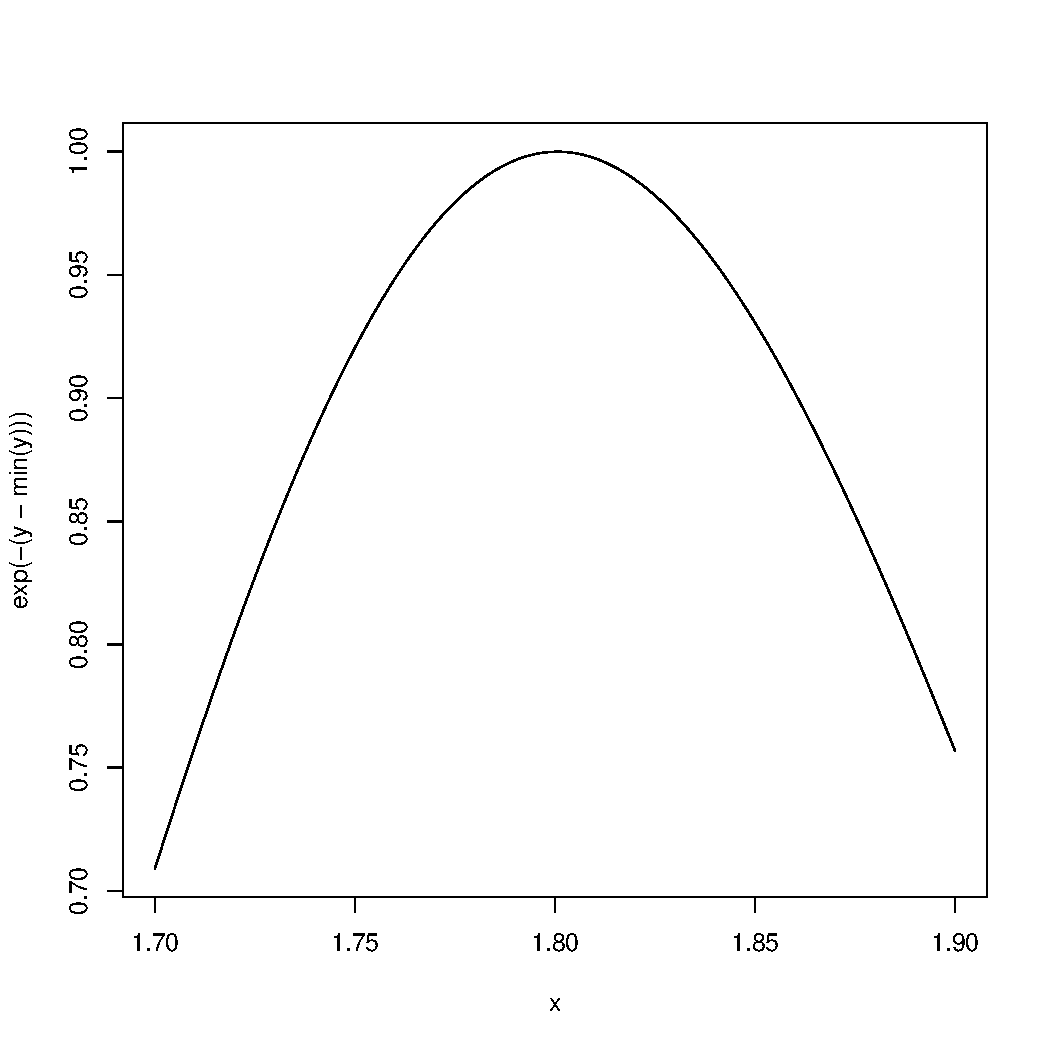
\includegraphics[width=\maxwidth]{figure/unnamed-chunk-93-1} 
\begin{kframe}\begin{alltt}
\hlstd{nLL} \hlkwb{<-} \hlkwd{make.NegLogLik}\hlstd{(normals,} \hlkwd{c}\hlstd{(}\hlnum{FALSE}\hlstd{,} \hlnum{2}\hlstd{))}
\hlstd{x} \hlkwb{<-} \hlkwd{seq}\hlstd{(}\hlnum{0.5}\hlstd{,} \hlnum{1.5}\hlstd{,} \hlkwc{len} \hlstd{=} \hlnum{100}\hlstd{)}
\hlstd{y} \hlkwb{<-} \hlkwd{sapply}\hlstd{(x, nLL)}
\hlkwd{plot}\hlstd{(x,} \hlkwd{exp}\hlstd{(}\hlopt{-}\hlstd{(y} \hlopt{-} \hlkwd{min}\hlstd{(y))),} \hlkwc{type} \hlstd{=} \hlstr{'l'}\hlstd{)}
\end{alltt}
\end{kframe}
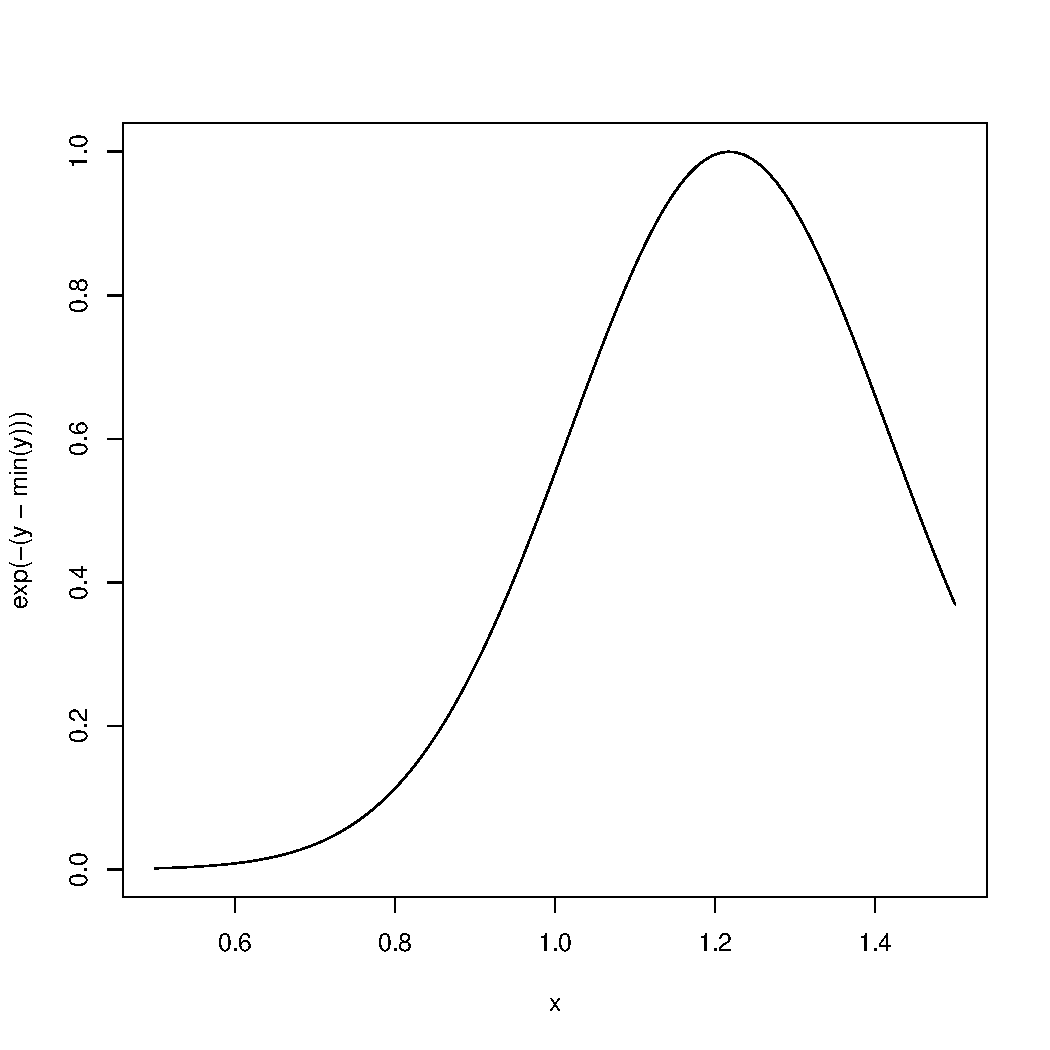
\includegraphics[width=\maxwidth]{figure/unnamed-chunk-93-2} 

\end{knitrout}
    
  \subsection{Resumen de ámbito léxico}
  \begin{itemize}
    \item Las funciones objetivo pueden ser "construidas", para que contengan todos los datos necesarios para evaluar la función
    \item No hay necesidad de llevar a todas partes largas listas de argumentos - útil para el trabajo interactivo y exploratorio.
    \item El código puede simplificarse y limpiarse
    \item Referencia: Robert Gentleman and Ross Ihaka (2000). “Lexical Scope and Statistical Computing,” \emph{JCGS}, 9, 491–508.
  \end{itemize}

\section{Normas de codificación en \texttt{R}}
\begin{enumerate}
  \item Siempre usar archivos de texto / editor de texto.
  \item Tabular el código
  \item Limitar el ancho del código(¿80 columnas?)
  \item Limitar la longitud de funciones individuales
\end{enumerate}

\section{Fechas y horas en \texttt{R}}
\texttt{R} ha desarrollado una representación especial de fechas y horas:
\begin{itemize}
  \item Las fechas se representan mediante la clase \texttt{Date}
  \item Las horas se representan mediante las clases \texttt{POSIXct} o \texttt{POSIXlt}
  \item Las fechas se almacenan internamente como el número de días desde 1970-01-01
  \item Las horas se almacenan internamente como el número de segundos desde 1970-01-01.
\end{itemize}

  \subsection{Fechas en \texttt{R}}
  Las fechas se representan mediante la clase \texttt{Date} y puede ser obligadas a convertirse en cadenas de caracteres usando la función \texttt{as.Date()}.
\begin{knitrout}
\definecolor{shadecolor}{rgb}{0.969, 0.969, 0.969}\color{fgcolor}\begin{kframe}
\begin{alltt}
  \hlstd{x} \hlkwb{<-} \hlkwd{as.Date}\hlstd{(}\hlstr{"1970-01-01"}\hlstd{)}
  \hlstd{x}
\end{alltt}
\begin{verbatim}
[1] "1970-01-01"
\end{verbatim}
\begin{alltt}
  \hlkwd{unclass}\hlstd{(x)}
\end{alltt}
\begin{verbatim}
[1] 0
\end{verbatim}
\begin{alltt}
  \hlkwd{unclass}\hlstd{(}\hlkwd{as.Date}\hlstd{(}\hlstr{"1970-01-02"}\hlstd{))}
\end{alltt}
\begin{verbatim}
[1] 1
\end{verbatim}
\end{kframe}
\end{knitrout}

  \subsection{Horas en \texttt{R}}
  Las horas se representan usando las clases \texttt{POSIXct} o \texttt{POSIXlt}
  \begin{itemize}
    \item \texttt{POSIXct} es sólo  un grán número entero, al fin de cuentas. Usa una clase cuando se quiere almacenar horas en algo como un data frame.
    \item \texttt{POSIXlt} es una lista que almacena una serie de información como el día de la semana, día del año, mes, día del mes.
  \end{itemize}
  
  Existe un número de funciones genéricas que trabajan con fechas y horas:
  \begin{itemize}
    \item \texttt{weekdays}: genera el día de la semana
    \item \texttt{months}: genera el nombre del mes
    \item \texttt{quarters}: genera el número del trimestre ("Q1", "Q2", "Q3" o "Q4")
  
  Las horas pueden ser obligadas a convertirse en una cadena de caracteres usando las funciones \texttt{as.POSIXct} o \texttt{as.POSIXlt}
  
  \end{itemize}
\begin{knitrout}
\definecolor{shadecolor}{rgb}{0.969, 0.969, 0.969}\color{fgcolor}\begin{kframe}
\begin{alltt}
  \hlstd{x} \hlkwb{<-} \hlkwd{Sys.time}\hlstd{()}
  \hlstd{x}
\end{alltt}
\begin{verbatim}
[1] "2015-12-22 18:39:54 COT"
\end{verbatim}
\begin{alltt}
  \hlstd{p} \hlkwb{<-} \hlkwd{as.POSIXlt}\hlstd{(x)}
  \hlkwd{names}\hlstd{(}\hlkwd{unclass}\hlstd{(p))}
\end{alltt}
\begin{verbatim}
 [1] "sec"    "min"    "hour"   "mday"   "mon"    "year"  
 [7] "wday"   "yday"   "isdst"  "zone"   "gmtoff"
\end{verbatim}
\begin{alltt}
  \hlstd{p}\hlopt{$}\hlstd{sec}
\end{alltt}
\begin{verbatim}
[1] 54.18555
\end{verbatim}
\end{kframe}
\end{knitrout}

  También es posible usar el formato \texttt{POSIXct}
\begin{knitrout}
\definecolor{shadecolor}{rgb}{0.969, 0.969, 0.969}\color{fgcolor}\begin{kframe}
\begin{alltt}
  \hlstd{x} \hlkwb{<-} \hlkwd{Sys.time}\hlstd{()}
  \hlstd{x} \hlcom{## Ya en formato 'POSIXct'}
\end{alltt}
\begin{verbatim}
[1] "2015-12-22 18:39:54 COT"
\end{verbatim}
\begin{alltt}
  \hlkwd{unclass}\hlstd{(x)}
\end{alltt}
\begin{verbatim}
[1] 1450827594
\end{verbatim}
\begin{alltt}
  \hlstd{x}\hlopt{$}\hlstd{sec}
  \hlstd{p} \hlkwb{<-} \hlkwd{as.POSIXlt}\hlstd{(x)}
  \hlstd{p}\hlopt{$}\hlstd{sec}
\end{alltt}
\begin{verbatim}
[1] 54.22062
\end{verbatim}
\end{kframe}
\end{knitrout}

  Finalmente, existe una función \texttt{strptime} en caso de que sus fechas estén escritas en diferente formato
\begin{knitrout}
\definecolor{shadecolor}{rgb}{0.969, 0.969, 0.969}\color{fgcolor}\begin{kframe}
\begin{alltt}
  \hlstd{datestring} \hlkwb{<-} \hlkwd{c}\hlstd{(}\hlstr{"January 10, 2012 10:40"}\hlstd{,} \hlstr{"December 9, 2011 9:10"}\hlstd{)}
  \hlstd{x} \hlkwb{<-} \hlkwd{strptime}\hlstd{(datestring,} \hlstr{"%B %d, %Y %H: %M"}\hlstd{)}
  \hlstd{x}
\end{alltt}
\begin{verbatim}
[1] "2012-01-10 10:40:00 COT" "2011-12-09 09:10:00 COT"
\end{verbatim}
\begin{alltt}
  \hlkwd{class}\hlstd{(x)}
\end{alltt}
\begin{verbatim}
[1] "POSIXlt" "POSIXt" 
\end{verbatim}
\end{kframe}
\end{knitrout}
  Es posible no recordar el formato de las cadenas. Revise \texttt{?strptime} para más detalles.
  
  \subsection{Operaciones con fechas y horas}
  Es posible usar operaciones matemáticas con fechas y horas. Realmente, sólo sumar y restar. También es posible hacer comparaciones (ej. ==, <=)
\begin{knitrout}
\definecolor{shadecolor}{rgb}{0.969, 0.969, 0.969}\color{fgcolor}\begin{kframe}
\begin{alltt}
  \hlstd{x} \hlkwb{<-} \hlkwd{as.Date}\hlstd{(}\hlstr{"2012-01-01"}\hlstd{)}
  \hlstd{y} \hlkwb{<-} \hlkwd{strptime}\hlstd{(}\hlstr{"9 Jan 2011 11:34:21"}\hlstd{,} \hlstr{"%d %b %Y %H:%M:%S"}\hlstd{)}
  \hlstd{x}\hlopt{-}\hlstd{y}
\end{alltt}


{\ttfamily\noindent\color{warningcolor}{Warning: Incompatible methods ("{}-.Date"{}, "{}-.POSIXt"{}) for "{}-"{}}}\begin{alltt}
  \hlstd{x} \hlkwb{<-} \hlkwd{as.POSIXlt}\hlstd{(x)}
  \hlstd{x}\hlopt{-}\hlstd{y}
\end{alltt}
\begin{verbatim}
Time difference of 356.3095 days
\end{verbatim}
\end{kframe}
\end{knitrout}

  Incluso un seguimiento de los años bisiestos, segundos bisiestos, el horario de verano y zonas horarias
\begin{knitrout}
\definecolor{shadecolor}{rgb}{0.969, 0.969, 0.969}\color{fgcolor}\begin{kframe}
\begin{alltt}
  \hlstd{x} \hlkwb{<-} \hlkwd{as.Date}\hlstd{(}\hlstr{"2012-03-01"}\hlstd{)}
  \hlstd{y} \hlkwb{<-} \hlkwd{as.Date}\hlstd{(}\hlstr{"2012-02-28"}\hlstd{)}
  \hlstd{x}\hlopt{-}\hlstd{y}
\end{alltt}
\begin{verbatim}
Time difference of 2 days
\end{verbatim}
\begin{alltt}
  \hlstd{x} \hlkwb{<-} \hlkwd{as.POSIXct}\hlstd{(}\hlstr{"2012-10-25 01:00:00"}\hlstd{)}
  \hlstd{y} \hlkwb{<-} \hlkwd{as.POSIXct}\hlstd{(}\hlstr{"2012-10-25 06:00:00"}\hlstd{,} \hlkwc{tz} \hlstd{=} \hlstr{"GMT"}\hlstd{)}
  \hlstd{y}\hlopt{-}\hlstd{x}
\end{alltt}
\begin{verbatim}
Time difference of 0 secs
\end{verbatim}
\end{kframe}
\end{knitrout}















\end{document}
  
